\documentclass[11pt]{report}

\usepackage[dutch]{babel}

% LAYOUT
\usepackage[margin=2.54cm]{geometry}
\usepackage{rotating}
\usepackage{pdflscape}
\usepackage{afterpage}
\usepackage{titlesec}
\usepackage{wrapfig}
%\usepackage[document]{ragged2e}
\rightskip=0pt plus2em\spaceskip=.3333em \xspaceskip=.5em\relax
% \hyphenpenalty=10000 \exhyphenpenalty=10000\relax

% TABLES
\usepackage{booktabs}
\usepackage{multirow}
\usepackage{xcolor}
\usepackage{tabularx}

% IMAGES
\usepackage{graphicx}

%table of contents
\usepackage{hyperref}
\hypersetup{
    colorlinks,
    citecolor=black,
    filecolor=black,
    linkcolor=black,
    urlcolor=black
}

\graphicspath{{res/img/}}

\usepackage[backend=biber,style=apa,autocite=inline]{biblatex}
\DeclareLanguageMapping{dutch}{dutch-apa}
\addbibresource{Satellite.bib}

\setcounter{secnumdepth}{3}


%%% DUTCH

\renewcommand{\chaptername}{Hoofdstuk}
\renewcommand{\figurename}{Figuur}
\renewcommand{\tablename}{Tabel}


\titleformat{\chapter}
  {\normalfont\LARGE\bfseries}{\thechapter}{1em}{}
\titlespacing*{\chapter}{0pt}{3.5ex plus 1ex minus .2ex}{2.3ex plus .2ex}

\begin{document}


	\begin{titlepage}
    \begin{center}
        \vspace*{1cm}
  
        \huge{\textbf{Afstudeerverslag}} \\ \vspace{0.2cm} \large 
        \large{\textbf{Satellite}} \\
        \vspace{0.2cm}
        \large
  
        Patrick de Jong \\
        \vfill
  
        \vspace{0.8cm}
    
    \end{center}
 \end{titlepage}
	\chapter*{Colofon}
\textbf{Document}
\begin{table}[h!]
	\begin{tabular}{p{5cm}l}
	Titel:           & Eindverslag  \\
	Opdracht:		 & Satellite  	\\
	Versie:          & 3.0          \\
	Datum:           & 18 juni 2021 \\
	\end{tabular}
\end{table}

\noindent\textbf{Auteur}
\begin{table}[h!]
	\begin{tabular}{p{5cm}l}
	Studentnaam:        & Patrick de Jong             \\
	Studentnummer:      & 2124986                     \\
	Email:              & pejong1@avans.nl            \\
	Telefoonnummer:     & +31621840073                \\
	Adres:				& Vinkenslag 8					\\
	Postcode:			& 4901 AP					\\
	Plaats:				& Oosterhout, Nederland		\\
	\end{tabular}
\end{table}

\noindent\textbf{Afstudeerbedrijf}
\begin{table}[h!]
	\begin{tabular}{p{5cm}l}
	Bedrijfsbegeleider: & Mark-Ivo van Ooijen         \\
	Email:              & mark-ivo@sensormaritime.com \\
	Bedrijf:            & Sensor Maritime             \\
	Adres:				& Nieuwe Linie 9			\\
	Postcode:			& 5146 PJ					\\
	Plaats:				& Vught, Nederland			\\
	\end{tabular}
\end{table}

\noindent\textbf{Onderwijsinstelling}
\begin{table}[h!]
	\begin{tabular}{p{5cm}l}
	Docentbegeleider 1: & Andries van Dongen          \\
	Email:              & ah.vandongen@avans.nl       \\
	Docentbegeleider 2: & Pieter Kop Jansen           \\
	Email:              & psm.kopjansen@avans.nl      \\
	School:             & Avans Hogeschool Breda      \\
	Adres:				& Lovensdijkstraat 61		\\
	Postcode:			& 4818 AJ					\\
	Plaats:				& Breda, Nederland			\\
	\end{tabular}
\end{table}
	\chapter*{Voorwoord}
Dit afstudeerverslag is het resultaat van het product Satellite. Dit product is ontwikkeld voor Sensor Maritime, waar ik de afgelopen 6 maanden mijn afstudeerstage heb gevolgd voor de studie Technische Informatica. De afstudeerstage is gevolgd op de afdeling Research \& Development met de rol software engineer. Dit document beschrijft het vooronderzoek, software ontwerp en implementatie van het product. Tijdens mijn afstudeerstage heb ik gekeken naar generieke software ontwerp in de embedded sector. \newline

\noindent Om te beginnen, wil ik mijn stagebegeleider, Mark-Ivo van Ooijen bedanken voor zijn hulp tijdens het project. Hij heeft me ondersteund tijdens het project bij problemen of vragen. Dit heeft me duidelijkheid over het project gegeven. Daarnaast heeft de samenwerking met Mark-ivo mijn analysekwaliteiten verbeterd. \newline 

\noindent Verder wil ik Andries van Dongen bedanken voor zijn ondersteuning als schoolbegeleider. Hij heeft kritisch gekeken naar mijn ingeleverde werk en heeft me feedback gegeven waar ik kon verbeteren. Met de hulp van zijn reviews zijn mijn zelfreflectie en evaluatie skills verbeterd. \newline

\noindent Patrick de Jong \newline
\noindent Oosterhout, vrijdag 18 juni 2021

	\chapter*{Samenvatting}
Sensor Maritime heeft een nieuw product ontwikkeld genaamd Satellite. Satellite is ontwikkeld om een universeel data-driven optimalisatie te maken voor kapiteins van binnenvaartschepen. Satellite is uniek omdat de kapitein plug and play verschillende sensoren kan toevoegen specifiek voor zijn binnenvaartschip. 

Voor de afstudeerstage is er gevraagd aan de stagiair om twee onderdelen te ontwikkelen. Ten eerste moet er gekeken worden naar generieke software ontwerp om verschillende sensoren makelijk en snel te ondersteunen. Vervolgens moet er ook gekeken worden naar verschillende 
{\color{red} \textbf{TOEVOEGEN}}


	\tableofcontents
	\listoffigures
	\begingroup
	\let\clearpage\relax
	\listoftables
	\endgroup
	\chapter{Inleiding}
Sensor Maritime heeft een nieuwe product ontwikkeld genaamd Satellite. Satellite is ontwikkeld om een universeel data-driven optimalisatie te maken voor kapiteinen van binnenvaartschepen. Satellite is uniek omdat de kapitein plug and play verschillende sensoren kan toevoegen specifiek voor zijn binnenvaartschip. Sensor Maritime heeft op dit moment alleen nog maar de hardware ontwikkeld. De vraag aan de stagair is om een generieke applicatie te ontwikkelen voor de hardware om verschillende sensoren te ondersteunen.\newline

\noindent Het project Satellite heeft het volgende hoofdvraag \textbf{Hoe kan een modulair software systeem worden ontwikkeld voor de Satellite hardware zo dat verschillende sensoren ondersteunt worden en data verstuurd kan worden naar een extern opslagpunt?} Om dit hoofdvraag zal er worden onderzocht naar generieke applicatie onwerp, stabiele communicatie en hardware validatie. Het product wordt onderzocht, implementeert, getest en uiteindelijk wordt er een demo gegeven. \newline


\noindent De volgende hoofdstukken komen aan te pas in het verslag. Ten eerste zal er een samenvatting gegeven van het eindverslag. Vervolgens is er een voorwoord toegevoegd, dit geeft een persoonlijk bericht van mijn eigen ervaringen. Daarnaast wordt in het voorwoord ook een dankwoord gegeven. Na het voorwoord wordt er een inleiding gegeven. Vervolgens wordt er basisinformatie gegeven over Sensor Maritime, hierin wordt beschreven wie Sensor Maritime is en wat ze doen. De probleemanalyse is het volgende hoofdstuk, hierin wordt de projectomschrijving, hoofdvraag, deelvragen, doelstellingen en eisen beschreven worden. Na de probleemanalyse komt de aanpak. De aanpak geeft informatie over hoe de project voltooid wordt. Na de aanpak komt de methode technieken, dit geeft informatie wat er nodig is en wat er gebruikt is om een succesvolle applicatie te maken. Vervolgens wordt er gekeken naar de ontwerp van de applicatie. Daarnaast wordt er gekeken naar het testen van de applicatie. De resultaat zal terugkoppelen op de deelvragen. Als laatste zal er een conclusie en aanbevelingen gegeven worden. Hier wordt teruggekoppeld op de hoofdvraag en deelvragen.
	\chapter{Over Sensor Maritime}
Sensor Maritime is een bedrijf dat zicht focust op research en development in de maritieme sector. Sensor Maritime is een van de vier bedrijven die deel uitmaken van de Sensor Groep, deze groep bestaat uit Sensor Maritime, Sensor BV, Sensor Partners, en Vision Partners. Wat deze bedrijven met elkaar gemeen hebben, is dat deze allemaal gefocust zijn op het ontwikkelen van nieuwe technologieën met verschillende sensoren. Sensor Maritime heeft een kantoor en is op het moment gebaseerd in Vught. Het bedrijf bestaat uit 4 mensen en heeft drie afdelingen:
\begin{enumerate}
	\item Sales
	\item Service
	\item Research en Development
\end{enumerate}
Tijdens de afstudeerstage zal de afstudeerder alleen betrokken zijn bij Research and Development.
\newline

\noindent Sensor Maritime is niet anders dan een sensor georiënteerd bedrijf, deze zijn specifiek gefocust op het ontwikkelen van sensorsystemen voor binnenvaartschepen. De klant van Sensor Maritime zijn dan ook kapiteinen van binnenvaartschepen \ref{fig:customer_sensor_maritime}.
\begin{figure}[h!]

	\centering
	\caption{Klant van Sensor Maritime}
	\label{fig:customer_sensor_maritime}
	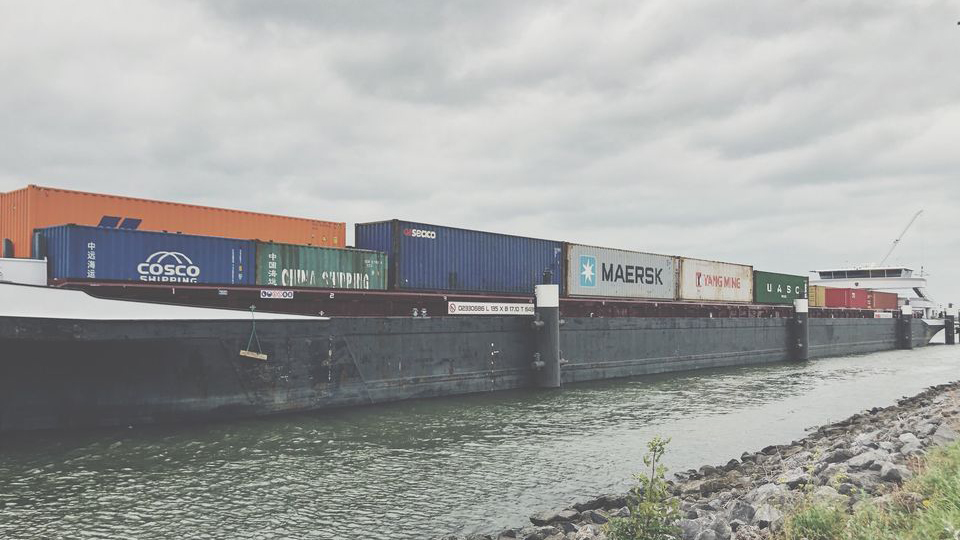
\includegraphics[width=0.7\linewidth]{about/binnevaart.jpg}
	

\end{figure}

\noindent Projecten waar Sensor Maritime momenteel bezig mee zijn is bijvoorbeeld, een systeem om objecten aan de zijkanten van een schip te kunnen detecteren en deze te tekenen op een scherm. Daarnaast is Sensor Maritime ook bezig met een systeem om objecten aan de voorkant van een schip te kunnen detecteren, en een systeem om te kunnen detecteren of een schip onder een brug door kan met de stuurhut.

	\chapter{Probleemanalyse}

\section{Probleemomschrijving}
Het project heet Satellite. Satellite is een nieuw project dat ontwikkeld wordt door Sensor Maritime in het kader van sensor data gedreven optimalisatie voor scheepvaart. Het geeft een kapitein de mogelijkheid om aan de hand van data kosten te besparen. Dit wordt gedaan door gegevens te verzamelen. Met deze data kan een kapitein efficiënter werken door veiliger, slimmer en duurzamer te opereren. Elke kapitein zal andere data willen voor zijn binnenvaartschip. Dit betekent dat het veranderen van sensoren simpel en snel moet zijn. Satellite (zie \ref{fig:shw} is zo ontwikkeld dat je plug \& play verschillende sensoren kan toevoegen. Dit wordt gedaan door verschillende IO porten en connectors toe te voegen aan de hardware. De Satellite hardware is al ontwikkeld, maar mist alleen nog de software om het als product te gebruiken. Aan de afstudeerder is  gevraagd om voor de hardware de applicatie te schrijven. Er moet nadruk gelegd worden bij de oplevering dat er een robuust en een generieke applicatie ontwikkeld wordt, die gefocust is op zowel de klant als de ontwikkelaar. Vervolgens is er ook gevraagd aan de afstudeerder om een systeem op te zetten dat toekomstige Satellite hardware snel en makkelijk getest kan worden.
\begin{figure}[h!]
	\begin{centering}

	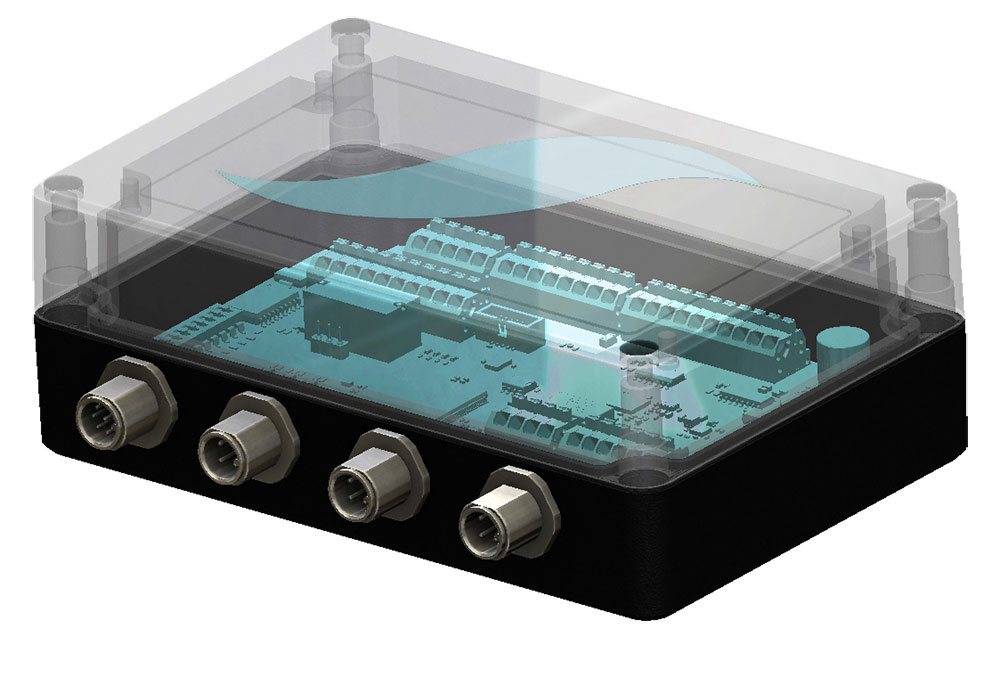
\includegraphics[width=0.35\linewidth]{statements/satellite.jpg}
	\caption{Satellite hardware}
	\label{fig:shw}
	\end{centering}
\end{figure}

\section{Betrokken partijen}
Tijdens de afstudeerstage zijn er twee partijen betrokken, Sensor Maritime in Vught en de student die de afstudeerstage volgt. Mark-Ivo van Ooijen van Sensor Maritime is de begeleider en projectleider. De tweede partij is de afstudeerder zelf, Patrick de Jong. Vanuit school zijn er ook twee examinatoren, maar deze zijn niet betrokken bij het project zelf. De examinatoren zijn Andries van Dongen, hij is de docentbegeleider die de afstudeerstage zal begeleiden. Pieter Kop Jansen zal er alleen zijn bij de uiteindelijke verdediging.

\section{Onderzoeksvraag}
De onderzoeksvraag tijdens de afstudeerstage is: \textbf{hoe kan een modulair softwaresysteem worden ontwikkeld voor de Satellite hardware zo dat verschillende sensoren ondersteund worden en data verstuurd kan worden naar één hoofdsysteem?}

\section{Deelvragen}
Het systeem moet robuust en makkelijk uitbreidbaar zijn. Daar sluiten dan twee van de deelvragen op aan. Bij een deelvraag is er gekeken naar de hardware validatie. Dit is een extra onderdeel wat Sensor Maritime aan de afstudeerder heeft gevraagd om een manier te ontwikkelen zodat er makkelijk nieuwe Satellite hardware getest kan worden.
\begin{enumerate}
	\item Hoe kan er een robuuste  communicatie gecreëerd worden tussen een hoofdsysteem en Satellite?
	\item Op welke manier moet de software ontworpen worden zodat het makkelijk uitbreidbaar is met nieuwe sensoren?
	\item Welke stappen zijn nodig om alle IO porten te testen van de Satellite?
\end{enumerate}

\section{Doelstellingen}
De doelstellingen van het project geven duidelijkheid in wat er precies bereikt moet worden in betrekking met de onderzoeksvraag en deelvraag. Dit is de lijst die de te bereiken doelstellingen aangeeft.
\begin{enumerate}
	\item De Satellite IO porten zijn volledig getest, en kunnen communiceren met sensoren.
	\item De Satellite heeft een robuuste communicatie over CAN en UDP. 
	\item De Satellite werkt met generieke en modulair opgebouwde software, waardoor het product in de toekomst makkelijk uitgebreid kan worden.
\end{enumerate}

\newpage
\section{Eisen}
Voor dat er een applicatie ontwikkeld kon worden is er besproken met de stagebegeleider waar de applicatie aan moet voldoen. De volgende tabel \ref{tab:eisen} geeft een overzicht van de eisen voor het project Satellite.
\begin{table}[h!]
	\centering
	\caption{MoSCoW Analyse}
	\label{tab:eisen}
	\begin{tabular}{lp{13cm}l}
	\toprule
	\textbf{ID} & \textbf{Eis} & \textbf{Prioriteit} \\ \midrule
	SM1			& Alle IO porten van de Satellite moeten getest worden 										& MUST	 \\
	SM2			& Implementatie van de hoekmeting en versnellingsassen 										& MUST	 \\ 
	SM3			& Spectrum analyse maken van de versnellingsassen 											& MUST	 \\ 
	SM4			& Errors moeten goed afgevangen worden, de applicatie mag niet crashen of blijven hangen 	& MUST	 \\ 
	SM5			& CAN-implementatie, en correct protocol afhandeling										& MUST	 \\ \midrule
	SM6			& Implementatie voor IO-Link sensoren 														& SHOULD \\
	SM7			& Hoogte sensoren en antenne sensor inlezen 												& SHOULD \\  \midrule
	SM8			& Standaard datastructuur voor packets die worden opgestuurd								& COULD	 \\
	SM9			& Debug berichten worden opgestuurd via UDP/CAN 											& COULD	 \\  \midrule
	SM10		& Ondersteuning van niet gekozen sensoren van Sensor Maritime 								& WON'T	 \\
	SM11		& Ondersteuning voor andere communicatiemiddelen dan UDP, CAN 								& WON'T	 \\
	SM12		& Ondersteuning voor andere embedded systemen  												& WON'T	 \\\bottomrule
	\end{tabular}
\end{table}

	\chapter{Aanpak} \label{ch:aanpak}

\section{Projectactiviteiten}
De afstudeerderstage is opgesplitst in verschillende fases, in dit hoofdstuk worden er voor elke fase de activiteiten geformuleerd. In de stage zijn er drie fases gespecificeerd. In de eerste fase zal gekeken worden naar het onderzoek, de implementatie, en uiteindelijk wordt het project afgerond. In de onderzoek fases wordt de criteria concreet gemaakt en wordt er gekeken naar de beste mogelijke implementatie van het gevraagde product. Na het onderzoek komt de ontwerp en implementatie fase, hier wordt het uiteindelijke product geïmplementeerd aan de hand van de onderzoek en criteria die in de vorige fase zijn opgesteld. Als de implementatie voltooid is komt de laatste fase, de afronding. In de afronding wordt er gekeken naar het uiteindelijke product aan de hand van de criteria.

\subsection{Onderzoek}
Tijdens de onderzoeksfase zal er een aantal stappen gemaakt worden om de het project af te bakenen en er wordt gekeken naar de implementatie van het project. Tijdens de stage komen de volgende activiteiten aanbod:
\begin{enumerate}
	\item Een onderzoek doen naar het ontwikkelen van een generiek applicatie, waarbij verschillende sensoren ondersteund kunnen worden.
	\item Een onderzoek doen naar payload ontwerp van de CAN-bus communicatie.
	\item Een onderzoek doen naar hardware validatie.
	\item Plan van aanpak
\end{enumerate}

\subsection{Implementatie}
In de implementatie fase worden de resultaten van de onderzoeksfase verwerkt in de applicatie. 
\begin{enumerate}
	\item Implementatie van het generieke software ontwerp
	\item Implementatie van de hardware validatie aan de hand van het testplan.
	\item Implementatie van het payload structuur van de CAN-bus communicatie.
\end{enumerate}

\newpage
\subsection{Afronding}
De afronding is de laatste fase van het project tijdens de afstudeerstage. In deze fase wordt er verwacht dat het product robuust en stabiel is en compleet genoeg om een demo te geven. In deze fase wordt de applicatie helemaal getest op eventuele bugs/glitches of incorrecte afhandeling van fouten. Daarnaast wordt er ook verwacht dat het eindverslag af voltooid is.
\begin{enumerate}
	\item Verwerken van het afstudeerverslag.
	\item De software wordt verder getest op eventuele bugs en glitches.
	\item Hardware validatie applicatie wordt vergeleken met het testplan.
\end{enumerate}


\section{Tussenresultaten}
Dit hoofdstuk laat zien de tussenresultaten van het project. De tussenresultaten wordt opgesplitst tussen milestones en documenten.

\subsection{Milestones}
In tabel \ref{tab:milestones} staan de milestones. Deze milestones zijn niet gelinkt aan documenten, maar juist aan de implementatie van het uiteindelijke product.
\begin{table}[h!]
		\caption{Milestones}
		\begin{tabular}{p{1cm}p{14cm}}
		\toprule
		\textbf{\#} & \textbf{Beschrijving} \\ \midrule
		1 & Software ontwerp om de generieke sensoren te ondersteunen      \\
		2 & Payload structuur ontwerp voor het CAN Bus protocol      \\
		3 & Implementatie applicatie aan de hand van het software ontwerp					\\
		4 & Hardware validatie geïmplementeerd		\\
		5 & Afronding ongeteste product \\
		6 & Afronding product              \\ \bottomrule
		\end{tabular}

	\label{tab:milestones}
\end{table}

\subsection{Documenten}
In tabel \ref{tab:documents} staan  alle documenten die door de afstudeerder zijn gemaakt, en welke documenten aan de Sensor Maritime geleverd wordt.
\begin{table}[h!] 
	\caption{Tussenresultaten van documenten}
	\begin{tabular}{p{1cm}p{14cm}}
	\toprule
	\textbf{\#} & \textbf{Documentnaam}   \\ \midrule
	1 & Definitief Plan van Aanpak afstuderen. \\
	2 & Onderzoeksdocument naar een generieke methode om sensoren te ondersteunen. \\
	3 & Document voor het payload structuur ontwerp voor het bestaande CAN Bus protocol \\
	4 & Testplan hardware validatie \\
	5 & Eindverslag afstuderen \\ \bottomrule
	\end{tabular}

\label{tab:documents}
\end{table}

\newpage
\section{Kwaliteit}
In dit hoofdstuk wordt er gekeken hoe de kwaliteit gewaarborgd wordt tijdens het project. Kwaliteit wordt onderverdeeld in verschillende hoofdstukken: het product en documentatie. Er wordt gekeken hoe de kwaliteit van het product het best gewaarborgd kan worden. Daarnaast bevordert dit een succesvolle afronding van de stage.

\subsection{Product}
De kwaliteit wordt bepaald door de klant en bedrijfsbegeleider. De afstudeerder is verantwoordelijk voor het product en zal de requirements opzetten met de bedrijfsbegeleider en klant. Met de requirements kunnen de milestones gedefinieerd worden. Met de hulp van de eisen en milestones wordt het project meetbaar en weet wat de klant uiteindelijk kan verwachten. \newline

\noindent Tijdens de implementatie is gebruik gemaakt van GitHub voor versiebeheer. Sensor Maritime heeft een eigen GitHub account waar alle projecten van Sensor Maritime opstaat. Met de hulp van Github kan er makkelijk gekeken worden hoe het project verloopt en code kan beoordeeld worden door de bedrijfsbegeleider. Op Github is een uiteindelijke release gemaakt voor prototypes. Aan het einde van de stage zal een final release gemaakt worden waar alles toegevoegd wordt. Hierin komt alle documentatie en informatie te staan om het project te kunnen bouwen en uploaden naar het hardware. Bij eventuele problemen kan de afstudeerder hulp vragen van de bedrijfsbegeleider om zo de kwaliteit te waarborgen. Er zal geen hulp komen van partijen die niet in het plan van aanpak zijn genoemd.

\subsection{Documentatie}
Net zoals het product zal de afstudeerder alle verantwoordelijkheid hebben voor de documentatie dat gemaakt is door de afstudeerder. Alle documenten worden in fases opgeleverd. Het conceptdocumenten zal bekeken worden door de bedrijfsbegeleider. De bedrijfsbegeleider zal hier opmerkingen geven en de afstudeerder zal deze opmerking verwerken voordat het opgestuurd wordt naar de docentbegeleider, de docentbegeleider is het laatste persoon die het document zal bekijken, de student zal alle opmerking verwerken wat een definitief document geeft. Alle versies van het documenten zal opgeslagen worden en zal uiteindelijk op OneDrive gezet worden volgens de richtlijnen van Sensor Maritime. De bedrijfsdocumenten worden niet in fases opgeleverd, de eerste versie van het bedrijfsdocument zal altijd een conceptverslag zijn.
	\chapter{Methode en technieken}
Dit hoofdstuk zal verschillende methode, technieken en tools beschrijven die gebruikt zijn tijdens het project. Voor elke tool zal er beschreven worden waarom voor een bepaalde methode, techniek en tool gekozen is. Er zal als eerst gekeken worden naar de methode, vervolgens de technieken en uiteindelijke de tools.

\section{Methode}
In het hoofdstuk wordt er gekeken naar alle methodes die gebruikt zijn tijdens het uitvoeren van het project. Daarnaast wordt er ook beschreven waarom ze gebruikt worden.

\subsection{HBO-I methodes}
Tijdens de afstudeerstage zal er gebruikt gemaakt worden van twee onderzoeksmethodieken, ten eerste zal er \textit{Hardware validation onderzoek} gebruikt worden voor de hardware validatie. De andere onderzoeksmethodiek is \textit{Design Pattern research}, dit zal gebruikt worden voor het generieke software ontwerp te ontwikkelen \parencite{researchmethods}. Hardware validation onderzoek is gekozen om een uiteindelijk testplan te ontwikkelen om het hardware te kunnen testen. Design Pattern research zal gebruikt worden om een duidelijk en generiek structuur van de applicatie te ontwikkelen. Hiervoor zal verschillende design patterns gebruikt worden. Voor de volgende deelvragen zal \textit{Design Pattern research} gebruikt worden: 
\begin{enumerate}
	\item De Satellite heeft een robuuste communicatie over CAN en UDP.
	\item Generiek en modulair opgebouwd software, waardoor het in de toekomst makkelijk uitgebreid kan worden.
\end{enumerate}

\noindent De laatste deelvraag zal beantwoord worden met \textit{Hardware validation onderzoek}:
\begin{enumerate}
	\item De Satellite IO porten zijn volledig getest, en kunnen communiceren met sensoren. Dit wordt gedaan aan de hand van een testplan.
\end{enumerate}

\subsection{Werkmethoden}
Om er voor te zorgen dat alle eisen en doelstelling gehaald worden is er van belang om te kiezen voor een goed werkmethode voor het project. Werkmethodes zorgen ervoor dat het project efficiënt en succesvol gedraaid worden. Er zijn verschillende werkmethodes bedacht, maar tijdens de stage is er een selectie gemaakt uit drie werkmethoden. De drie werkmethode zijn V-Model, waterval en Agile. Deze drie zijn gekozen omdat de stagiair hier al ervaring mee heeft. Dit betekent dat er geen nieuwe methodes geleerd hoeven te worden. \newline

\noindent Uiteindelijk is er gekozen voor een combinatie tussen Waterval en Agile. Dit is omdat er vaste eisen en taken zijn gespecificeerd door de klant in het begin van het project, die heel makkelijk opgesplitst kunnen worden in kleinere taken. Hierdoor zijn er weinig onzekerheden binnen het project en kon er waterval methode gekozen om het proces goed navolgbaar en meetbaar te maken. Van de waterval methode worden fases meegenomen die gaan als volgt. Als eerst komt de requirements, design, implementatie, verificatie en maintenance. De maintenance fases zal buiten de scope van het stage vallen. Er is gekozen voor Agile aangezien het niet duidelijk vanaf het begin welke taak als eerst geïmplementeerd moet worden. Dit zal dan besproken worden elke twee weken, en meerdere keren per week zal er besproken worden hoe de voortgang is.




\section{Technieken}
Er is als eerst gekeken naar een van de belangrijkste techniek van softwareontwikkeling, de programmeertaal. Elke taal heeft zijn voordelen en nadelen, er moet dus ook goed bekeken worden of een taal wel gebruikt kan worden voor embedded softwareontwikkeling. In Sensor Maritime worden een aantal talen standaard gebruikt, dat is C en C\#. Omdat het product in de toekomst nog aangepast kan worden is er niet gekeken naar andere talen zoals bijvoorbeeld Rust. Hiervoor is gekozen omdat de toekomstige developer deze taal dan zou moeten kennen. De hardware abstractie laag van de microcontroller is standaard geschreven in C. C is een low level taal wat ontwikkeld is voor verschillende doeleinden. Een van die doeleinden is om low level code te schrijven. Door de low level doeleinden kan er makkelijk manipulatie gedaan van de hardware. Daarnaast levert de Infineon IDE standaard een C compiler. Dit is een voordeel aangezien de compiler geoptimaliseerd is voor de Infineon's microcontroller. Met C zal dan uiteindelijke ook implementatie gedaan worden. Er is niet gekeken voor externe compilers voor ARM based systemen (ARM is een microcontroller architectuur) aangezien je dan niet weet wat de ondersteuning, en robuustheid ervan is. Daarnaast was ook gekeken naar de C++, aangezien het embedded systeem het standaard ondersteund, maar omdat binnen Sensor Maritime meer ervaring is met C, is er voor C gekozen. 

\section{Tools}
Tijdens de afstudeerstage zijn er een aantal verschillende tools gebruikt voor de implementatie en ontwerp van het project. De tools zijn opgesplitst in het ontwerp en implementatie van de software.

\subsection{Ontwerp}
\begin{enumerate}
	\item Visual Paradigm \\ Hiermee is verschillende UML-diagrammen ontwikkeld, zoals de klasse diagram en statemachines.
\end{enumerate}
\subsection{Implementatie}
\begin{enumerate}
	\item DAVE \\ DAVE is de standaard gemaakte IDE van Infineon, het heeft dus ook hardware abstractie support in de vorm van APPS, waardoor je de hardware makkelijk kan configureren.
	\item GitHub (Git) \\ Het standaard versiebeheer wat Sensor Maritime gebruikt.
	\item Segger J-Link \\ Met de J-Link kon er gebruikt gemaakt worden van debuggen, dit betekent dat dat je makkelijk weet waar het programma mee bezig is.
	\item Trello \\ De agile bord waarop alle sprints en taken bijgehouden wordt.
\end{enumerate}


	\chapter{Ontwerp}
In dit hoofdstuk wordt er gekeken naar het softwareontwerp, er wordt gefocust om een robuust en generiek applicatie en communicatie ontwikkelen. De applicatie op het moment opgebouwd in verschillende onderdelen, deze onderdelen zijn de applicatie, preprocessor, sensor drivers en abstractie en communicatie.

\section{Structuur}
Voor dat er gekeken kan worden naar het ontwerp moet er een worden gemaakt hoe de applicatie uiteindelijk zich moet gaan gedragen. Hoe moet er gecommuniceerd worden, hoe kiest de applicatie welke sensor hij aan het uitlezen is dit. De volgende afbeelding geeft \ref{fig:appstructuur}. 
\begin{figure}[h!]
	\centering
	\label{fig:appstructuur}
	\caption{Algemene structuur van de applicatie}
	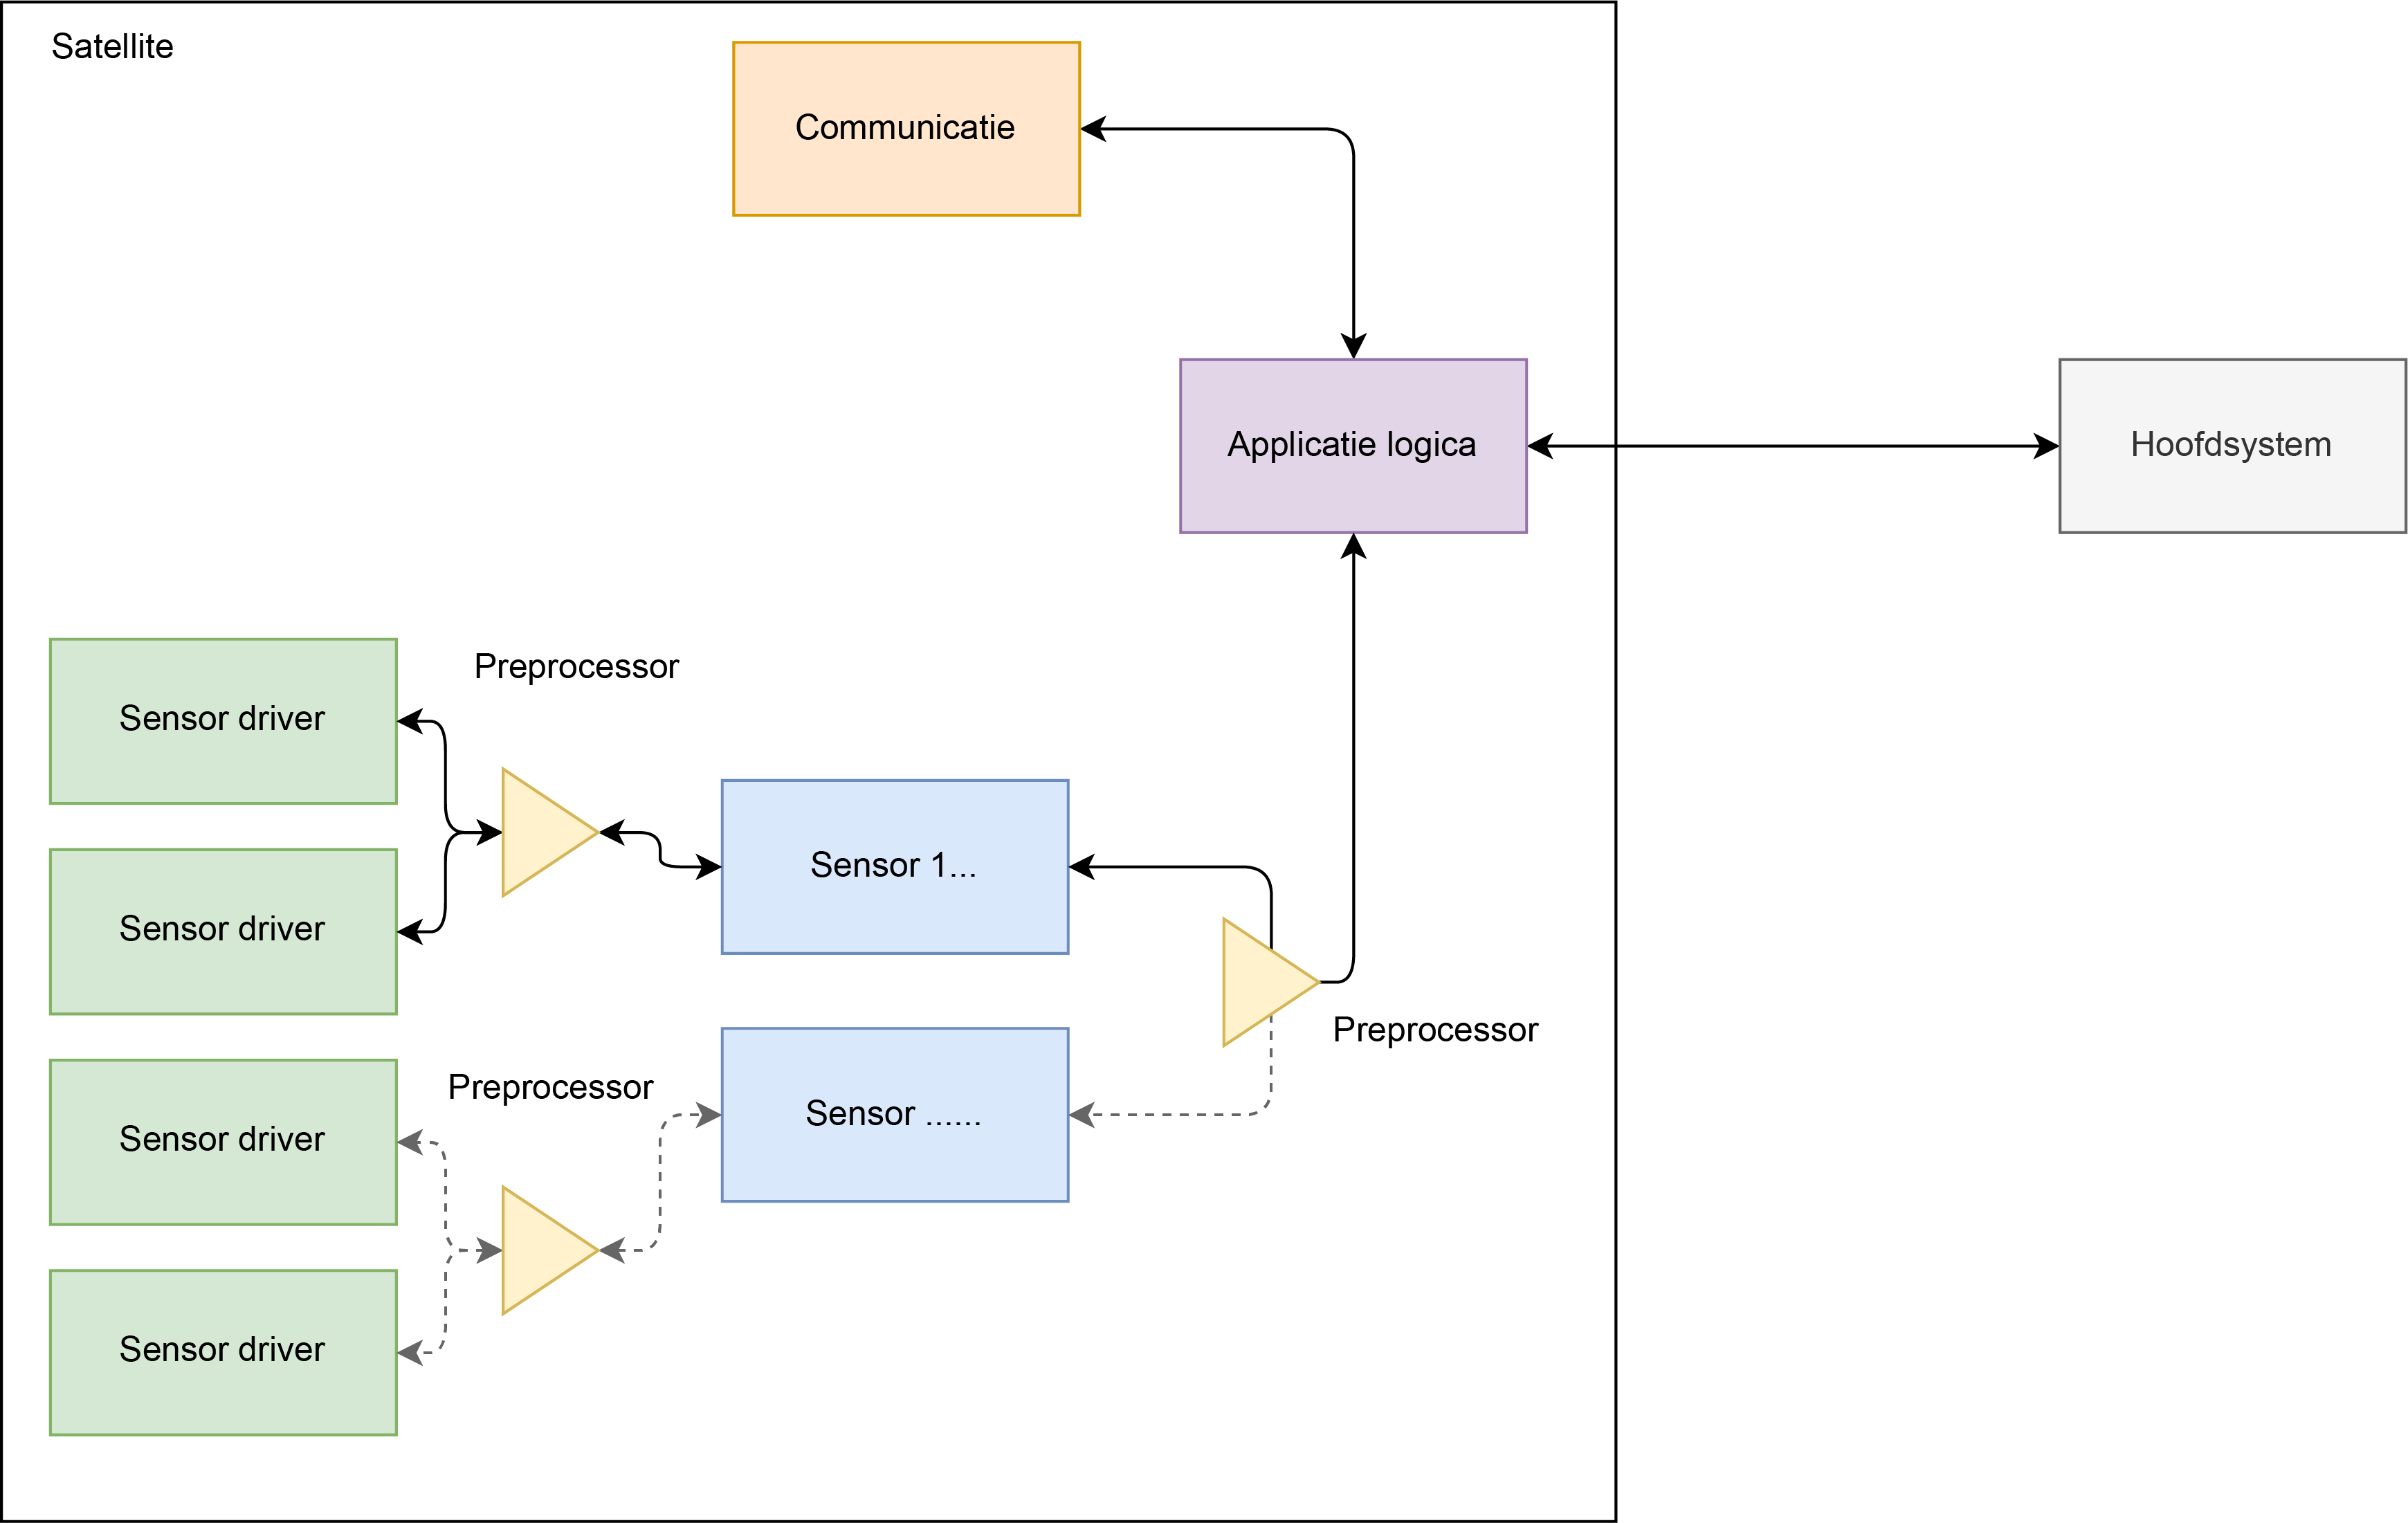
\includegraphics[width=1\linewidth]{ontwerp/compleet structuur.png}
\end{figure}

\newpage
\section{Applicatie}
De applicatie moet zo generiek mogelijk zijn, dit betekent dat de applicatie moet werken als er bijvoorbeeld van sensor verandert of toegevoegd wordt. Als er nieuwe sensor toegevoegd wordt is er een doel, het doel is dat de enige toevoeging wat er gemaakt moet worden is dat er een driver geschreven wordt voor dat specifieke sensor, maar aanpassing aan de applicatie moet minimaal gebeuren. In afbeelding \ref{fig:appontwerp} wordt een algemeen overzicht gemaakt hoe de applicatie in lagen is opgebouwd. 
\begin{figure}[h!]
	\centering
	\label{fig:appontwerp}
	\caption{De applicatie ontwerp in lagen}
	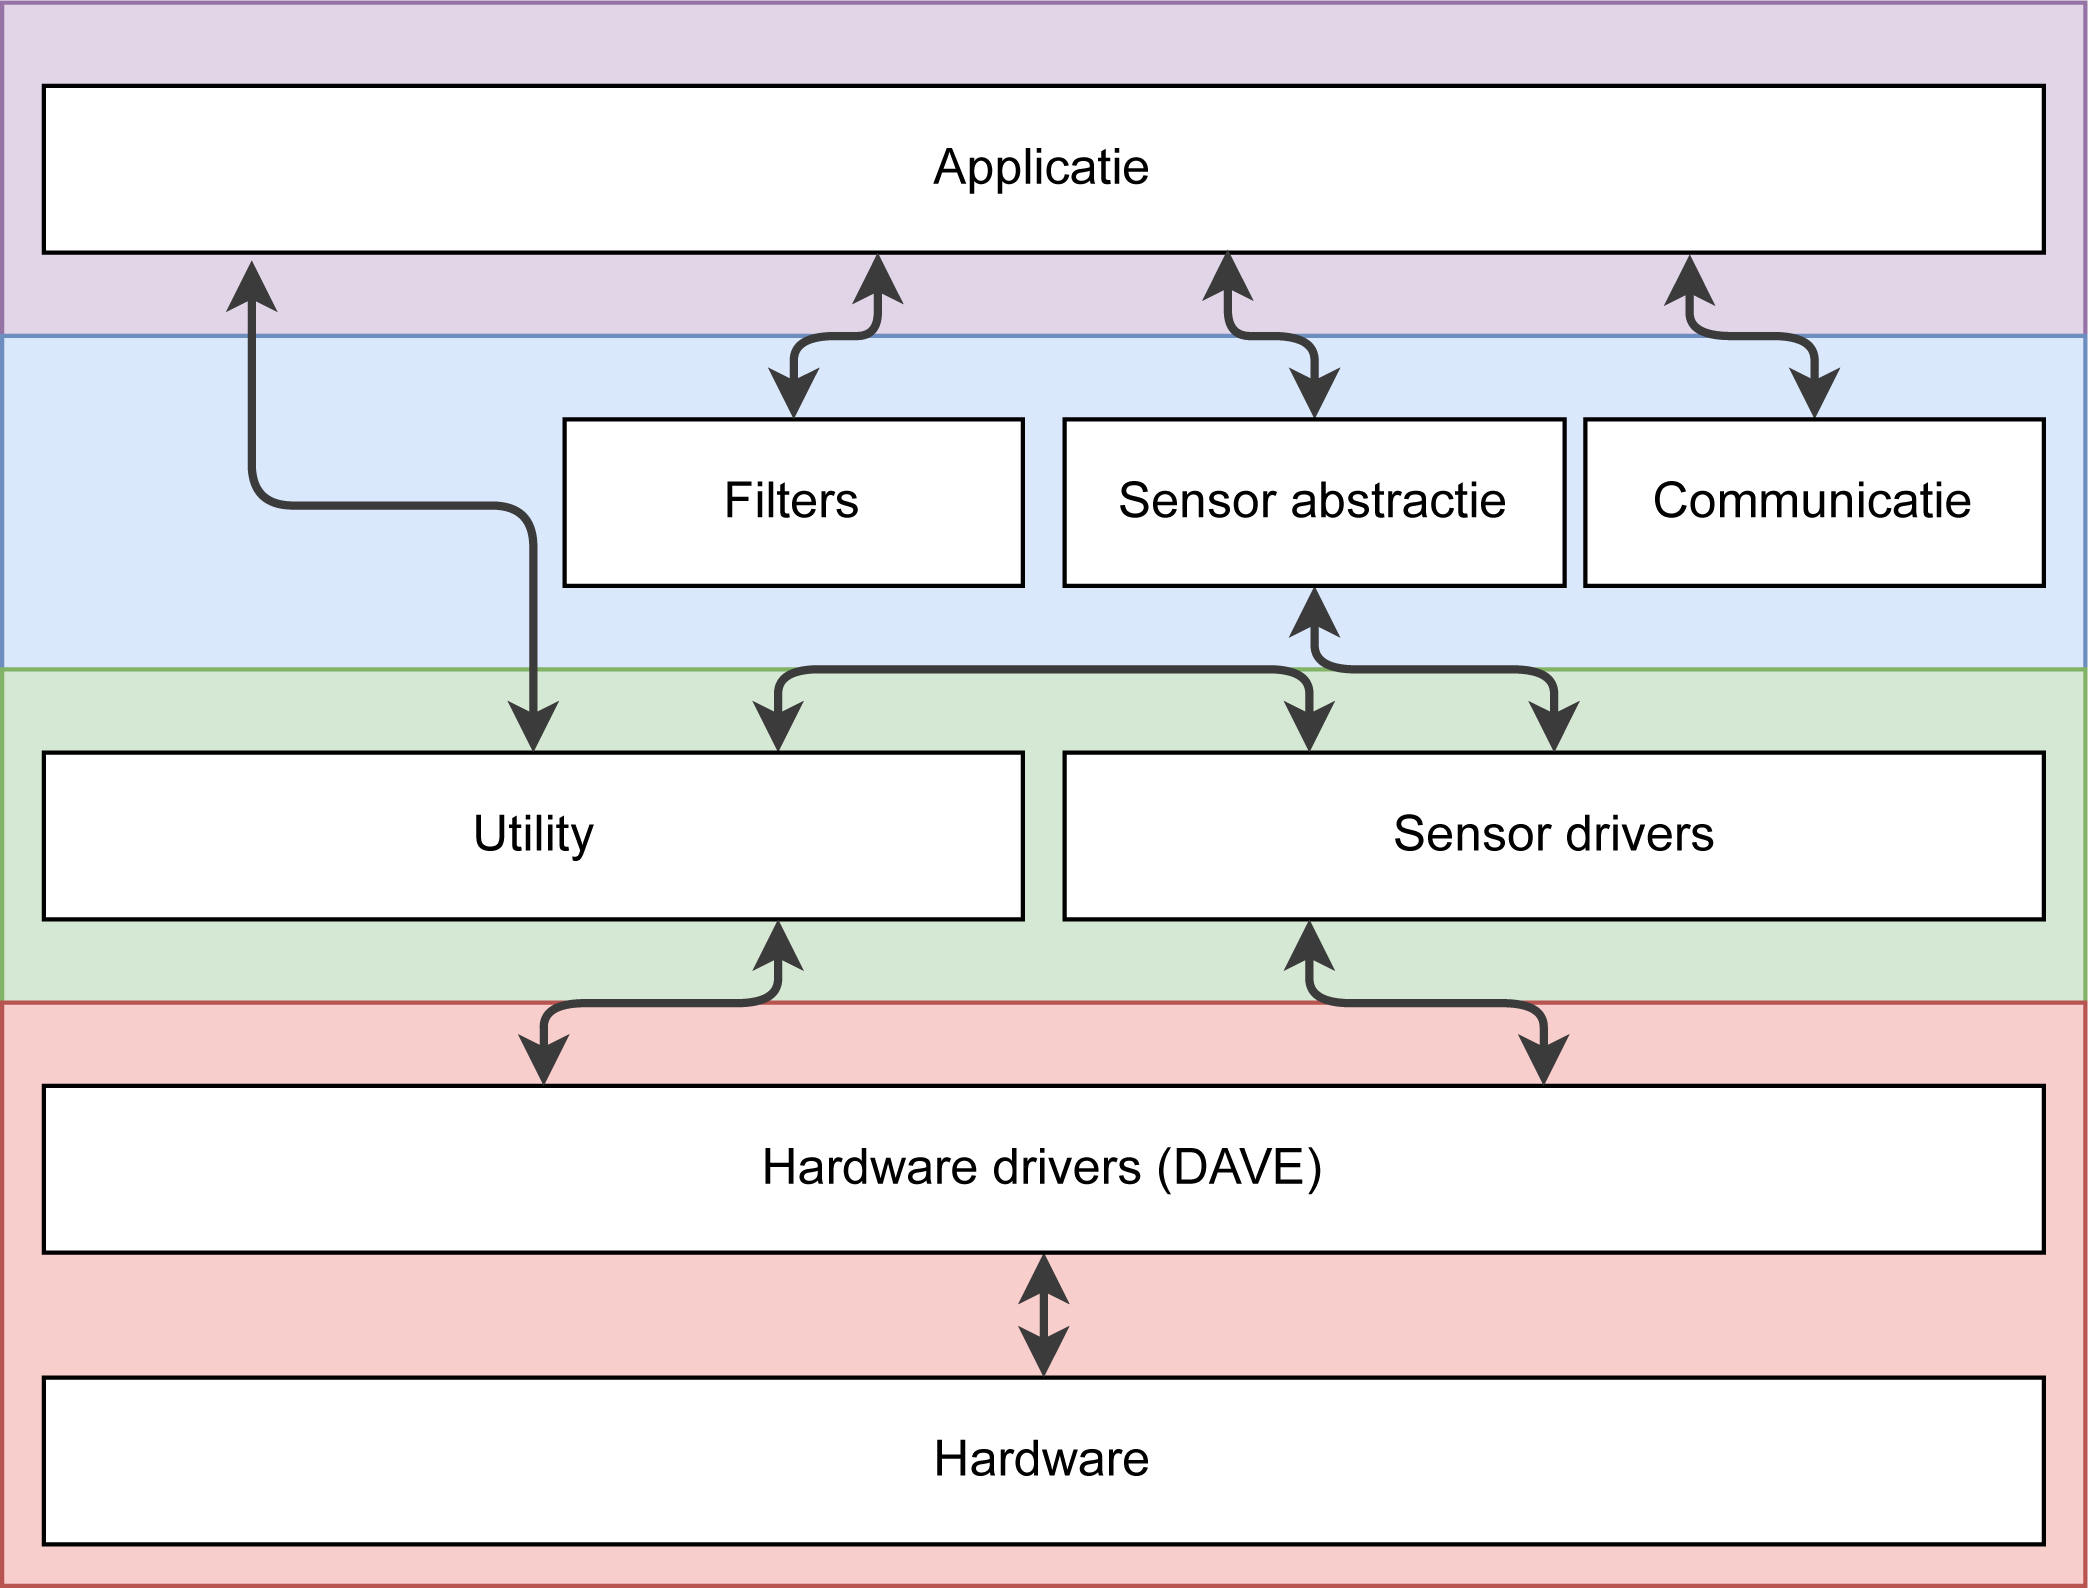
\includegraphics[width=1\linewidth]{ontwerp/applicatie/structuur.jpg}
\end{figure}



\subsection{Applicatie states}
De applicatie is zo ontworpen dat er gebruikt gemaakt wordt van verschillende states en taken die om de bepaalde tijd uitgevoerd moet worden. Deze states zijn tijdvariant maar sommige states zijn juist weer tijdsinvariant. Een tijdvariant taak  betekent dat om zoveel milliseconden er een taak uitgevoerd zal worden. In het ontworpen systeem wordt er om de 100 ms een akkoord gegeven aan de applicatie om sensor data op te halen en uiteindelijk opgestuurd te worden. Een belangrijk onderdeel van de applicatie is de communicatie, het is ontworpen dat er om de seconden sensor data opgestuurd wordt via UDP. Een tijdsinvariant taken zijn taken die niet op tijd gebaseerd zijn. De GNSS Sensor stuurt bijvoorbeeld continue data op. Dit betekent dat er verschillende taken zijn die uiteindelijke allemaal samengevoegd moet worden, hieronder is te zien \ref{fig:appstates} hoe de applicatie dit oplost.

\begin{figure}[h!]
	\centering
	\label{fig:appstates}
	\caption{Applicatie states van de applicatie}
	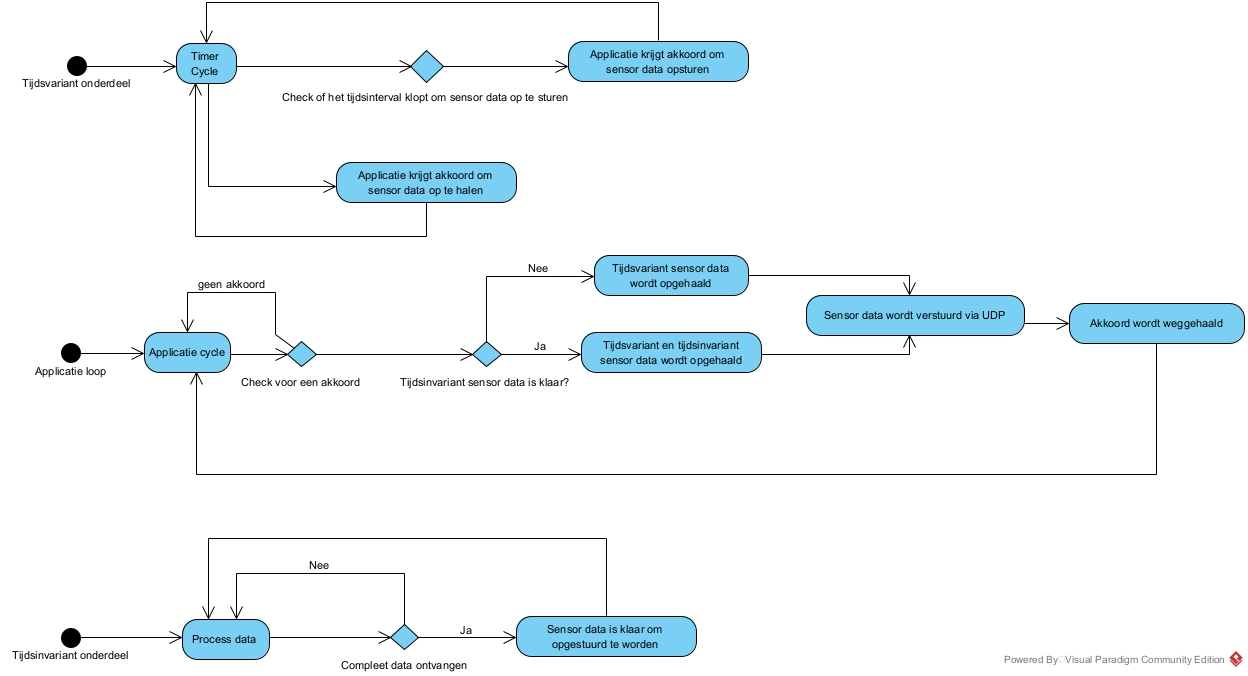
\includegraphics[width=0.73\linewidth]{ontwerp/applicatie/ApplicationStates.jpg}
\end{figure}

\noindent In het figuur \ref{fig:appstates} zijn er een aantal start nodes, ten eerste is de tijdsvariant onderdeel. Dit wordt per 100 milliseconden uitgevoerd, er wordt hier alleen gecheckt of de applicatie sensor data mag ophalen of verzenden. De applicatie krijgt om de 100 milliseconden dus de tijd om een signaal te geven aan de applicatie loop dat het tijdvariant sensor data mag op halen. Er mag pas data opgestuurd worden als een bepaald tijdsinterval gehaald wordt, het ontworpen systeem heeft op 1 seconden staan. Dit betekent voor 10 timer cycles mag er een keer data opgestuurd worden. Bij de 10de cycle wordt er weer signaal gegeven aan de applicatie loop dat er data opgestuurd mag worden. \newline

\noindent Naast het tijdsvariant onderdeel is er ook een tijdsinvariant onderdeel. Dit wordt gebruikt voor sensoren die bijvoorbeeld continue data opsturen naar de Satellite. Dit onderdeel slaat alleen data en als het een compleet sensor packet heeft dan geeft het een signaal aan de applicatie dat er een sensor packet verstuurd kan worden. \newline

\noindent Het laatste onderdeel is de applicatie loop, hier wordt de tijdvariant sensor data opgehaald en uiteindelijk opgestuurd. Er wordt als eerst gecheckt of er een akkoord is om sensor data op te halen of te versturen, als die er is dan haalt hij de tijdsvariant data op, en vervolgens wordt er gekeken of er een tijdsinvariant sensor packet klaar staat. Als dat is wordt het tijdsinvariant packet opgehaald, en opgestuurd via UDP. Mocht dit niet zijn dan wordt alleen het tijdsvariant sensor data opgehaald en gelijk opgestuurd. \newline

\section{Preprocessor} \label{sec:preprocessor}
De preprocessor is een handig onderdeel van de C taal en een belangrijk onderdeel van het project. De preprocessor is een stap wat voor het compileren gebeurt wordt, met bepaalde definities in de code kunnen sommige onderdelen niet gecompileerd worden of juist wel. Dit betekent dat makkelijk onderdelen uitgezet kan worden, bijvoorbeeld een specifieke sensor hoeft niet gebruikt te worden, normale wijze zou je dan een if statement bijvoorbeeld maken maar dit kan dan nu met de preprocessor. Dit betekent alleen wel dat alle code mee gecompileerd zou worden. Met de preprocessor voeg je weer een if statement toe maar dan hoeft de code niet aangepast te worden, er hoeft alleen maar definitie te verwijderen of toe te voegen. Dit betekent dat hele stuk logica niet weggehaald hoeft te worden, de preprocessor bepaald dan of bepaalde onderdelen gecompileerd worden of niet, dit verminderd de compilatie tijd en de uiteindelijk grootte van het programma \autocite{preprocessor}. 

\section{Sensor drivers en abstractie}
Voor de sensoren zijn er twee lagen ontwikkeld, namelijk de drivers en de abstractie. Dit is opgesplitst om de software zo generiek mogelijk te maken. Er wordt dan ook hier naar de volgende deelvraag bekeken \textbf{Op welke manier moet de software ontworpen worden zodat het makkelijk uitbreidbaar is voor nieuwe sensoren?} \newline 

\noindent De drivers en abstractie zijn opgesplitst zodat de applicatie structuur niet aangepast hoeft te worden, er zal dan alleen een nieuwe driver geschreven moeten worden en de abstractie aangepast moeten worden. De driver communiceert met de sensor, en de abstractie is de tussenpersoon tussen applicatie logica en driver. De applicatie zal dan niet veranderen. Om een voorbeeld te geven, de applicatie heeft een poll timer. Deze timer haalt om de 100 milliseconden data op van de inertial measurement unit. Mocht Sensor Maritime een nieuwe inertial measurement unit ondersteunen, normaal zou dan de applicatie logica ook aangepast moeten worden bepaalde met sensor drivers functies. De sensor abstractie vervangt dit het idee is dan ook dat in toekomst de applicatie laag code zo min mogelijk aangepast moet worden. De sensor abstractie moet dan juist aangepast worden en de applicatie laag roept dan de sensor abstractie code op. Hieronder is een overzicht \ref{fig:SensorAbstractie} te zien hoe het dan zou werken. De sensor keuze wordt makkelijk gedaan met de preprocessor (zie hoofdstuk \ref{sec:preprocessor}), hiermee worden sommige sensoren niet gecompileerd of juist wel.
\begin{figure}[h!]
	\centering
	\label{fig:SensorAbstractie}
	\caption{Sensor abstractie activity diagram}
	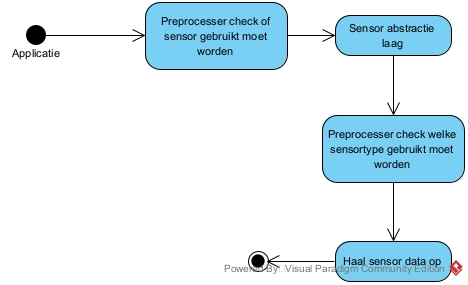
\includegraphics[width=0.46\linewidth]{ontwerp/applicatie/SensorAbstractie.jpg}
\end{figure}
	
	
\newpage
\section{Communicatie}
De Satellite heeft verschillende communicatiemiddelen, onder anderen ethernet en CAN Bus. Er zal gefocust worden op communicatie via CAN Bus aangezien dit het meest complex opgebouwd is.  De communicatie via CAN moet voldoen aan de volgende deelvraag: \textbf{Hoe kan er een robuuste communicatie gecreëerd worden tussen het hoofdsysteem en Satellite?} Er moet gekeken worden hoe dit stabiel en robuust gedaan kan worden.\newline


\noindent CAN is een groot onderdeel van de Sensor Maritime infrastructuur. De CAN-communicatie wordt gebruik om te kunnen communiceren met het hoofdsysteem. Hiervoor wordt een master en slave configuratie gebruikt. Het hoofdsysteem is de master en de Satellite en andere eindsystemen zullen dan de slave zijn. De master bepaalt hoe een slave apparaat zich gaat gedragen. CAN staat voor controlled area network, en maakt gebruik van een broadcast systeem. Dit betekent dat alle eindsystemen alle berichten ontvangen, De master kan niet specifiek naar een slave data sturen \autocite{can}. \newline

\noindent Sensor Maritime heeft een eigen protocol ontwikkeld wat gebouwd is op het CAN Bus protocol. Dit zal deels aangepast moeten worden om de Satellite sensoren te kunnen ondersteunen. Het huidige protocol is in afbeelding \ref{fig:canprotocol} te zien. Het protocol is opgebouwd uit velden wat uit 1 of 2 bytes bestaat. In tabel \ref{tab:cansensorprotocol} wordt beschreven wat de taak is van elk veld.
\begin{figure}[h!]
	\centering
	\label{fig:canprotocol}
	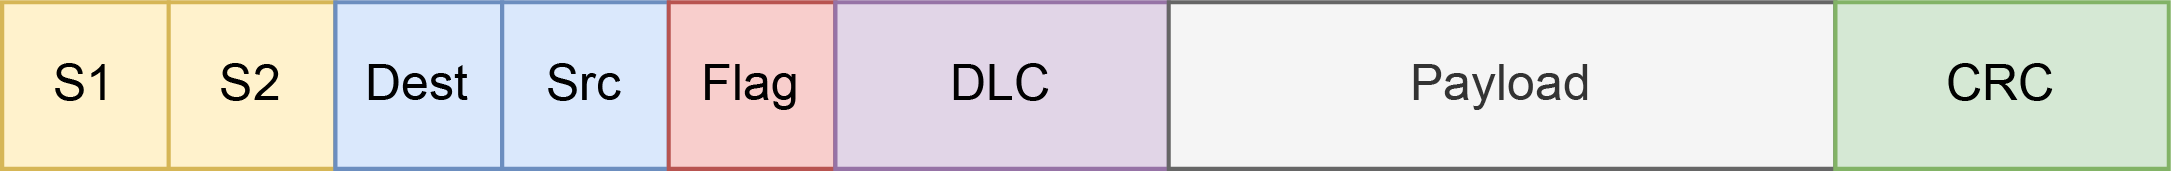
\includegraphics[width=0.75\linewidth]{voorstudie/communicatie/can.png}
	\caption{Sensor Maritime CAN protocol}
\end{figure}

\begin{table}[h!]
	\caption{Sensor Maritime CAN protocol opbouw}
	\label{tab:cansensorprotocol}
	\begin{tabular}{p{1.5cm}p{11.5cm}p{3cm}}
	\toprule
	\textbf{Blok} & \textbf{Beschrijving} & \textbf{Waarde}\\ \midrule
	S1		& De eerste start byte, dit geeft de start aan van het CAN bericht en wordt gebruikt voor herkenning, dit is een vaste waarde.	& 0x40 \\
	S2		& De tweede start byte, dit geeft de start aan van het CAN bericht en wordt gebruikt voor herkenning, dit is een vaste waarde. & 0x02 \\
	Dest	& Deze byte beschrijft voor wie het bericht bedoeld is.		& Verschillend per apparaat. \\
	Src		& Deze byte beschrijft van welke apparaat het bericht komt	& Verschillend per apparaat.\\ 
	Flag	& Dit geeft aan wat voor type bericht het is.             & 0 voor commando \\ 
			& & 1 voor request \\ 
	DLC		& DLC is een afkorting voor Data Length Code.             & \\ 
	Payload	& De data, dit verschillende aan de hand van de flag. & Verschillend per bericht\\
	CRC		& CRC staat voor Cyclic Redundancy Check, dit beschrijft hoe groot het bericht is wat verstuurd wordt. Hiermee kan de ontvanger valideren of het juiste is ontvangen. & Verschillend per bericht\\ \bottomrule
	\end{tabular}
\end{table}

\newpage
\subsection{Probleemstelling}
De huidige CAN BUS protocol ondersteunt de Satellite nog niet. De Satellite is een universeel systeem, waarmee verschillende sensoren verbonden zijn. Het huidige protocol is zo opgebouwd dat er maar één payload opgestuurd kan worden. Dit betekent dat als de Satellite twee sensoren op wil sturen het in de payload gestopt moet worden. Hiervoor moet een vaste structuur bepaald worden zodat de ontvanger weet wat er ontvangen wordt. Om dit probleem op te lossen zal er een aanpassing gemaakt moeten worden aan de bestaande CAN-protocol payload van Sensor Maritime. Hiervoor zijn verschillende oplossingen bedacht die hieronder worden beschreven. Uiteindelijk wordt toegelicht welke oplossing gekozen wordt en waarom. Voor alle payload structuren die beschreven worden zal er gebruik gemaakt worden van hetzelfde voorbeeld. Voor de voorbeelden worden er twee sensoren gebruikt die de Satellite zal ondersteunen. Deze twee sensoren zijn de inductie sensor en de altimeter sensor. De sensoren zullen gerepresenteerd worden als een getallen-lijst die begint bij 0. In het huidige systeem zijn er maar twee sensoren. Dit kan in de toekomst uitgebreid worden. Tabel \ref{tab:SensorRep} geeft een overzicht van de huidige sensoren en hun identificatie.

\begin{table}[h!]
	\centering
	\caption{Sensor identificatie representatie}
	\label{tab:SensorRep}
	\begin{tabular}{p{4cm}p{6cm}}
	\toprule
	Identificatie & Sensor        \\ \midrule
	0      & Inductor  \\
	1      & Altimeter \\ \bottomrule
	\end{tabular}%
\end{table}

\subsection{Structuur 1}
De eerste structuur is ontworpen om zo simpel mogelijk te zijn. Het idee bij dit ontwerp is dat er een identificatie is wat de sensor aangeeft en vervolgens gelijk de waarde van de sensor. Daarnaast voegt dit ook maar 1 byte toe aan de payload per sensor. Dit betekent dat het totale packet maar een aantal bytes groter zal zijn. De afbeelding \ref{fig:Structure1} geeft de opbouw en een voorbeeld weer, hierbij zijn twee sensoren te zien met de identificatie en de waarden van de sensor.
\begin{figure}[h!]
	\centering
	\label{fig:Structure1}


	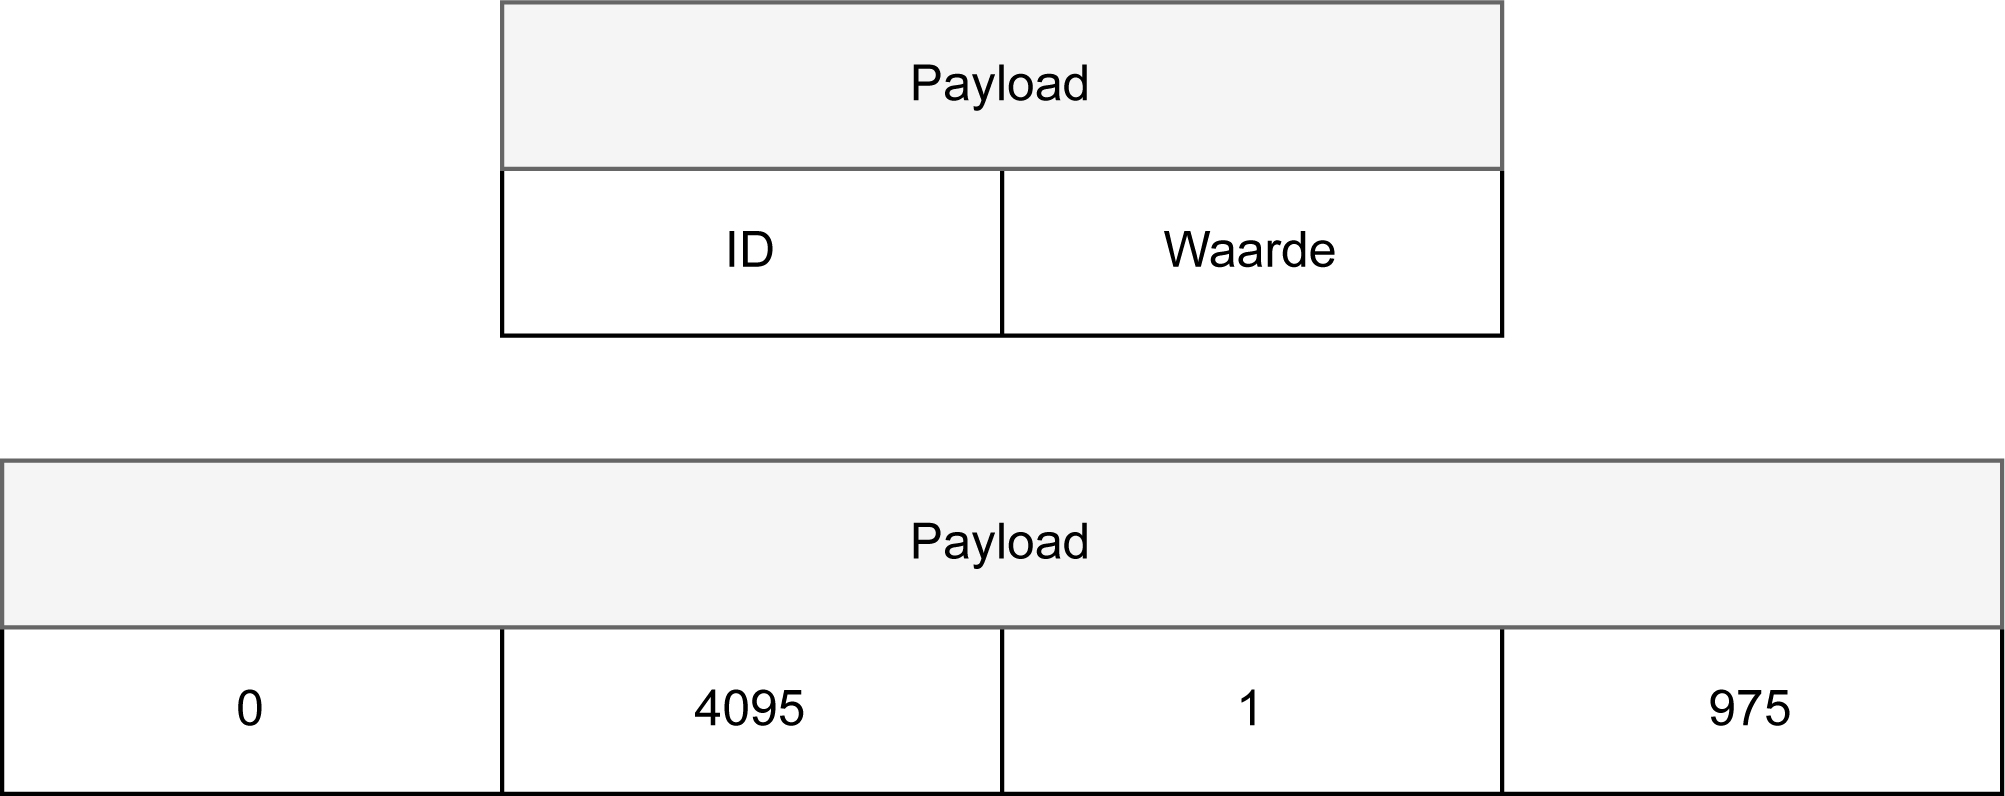
\includegraphics[width=0.75\linewidth]{voorstudie/communicatie/PayloadStructure1-01.jpg}
	\caption{Opbouw en voorbeeld van de payload structuur 1}
\end{figure}

\newpage
\subsection{Structuur 2}
Structuur 2 is opgezet om zoveel mogelijk te ondersteunen. Ten eerste ondersteunt dit meerdere datatypes, bijvoorbeeld 8, 16, 32 bit nummers maar ook 32 bit en 64 bit decimalen. Ten tweede geeft deze structuur duidelijk aan wat de grootte is van een packet. Packet grootte, geeft aan de hele sensor packet grootte in bytes. De identificatie geeft aan wat voor sensor het is. Dan komen er drie kolommen voor de waarde. Eerste wordt de waarde grootte in bytes gegeven, dan de waardetype en uiteindelijk de waarde zelf. In de volgende afbeelding \ref{fig:Structure2} is een overzicht te zien.
\begin{figure}[h!]
	\centering
	\label{fig:Structure2}

	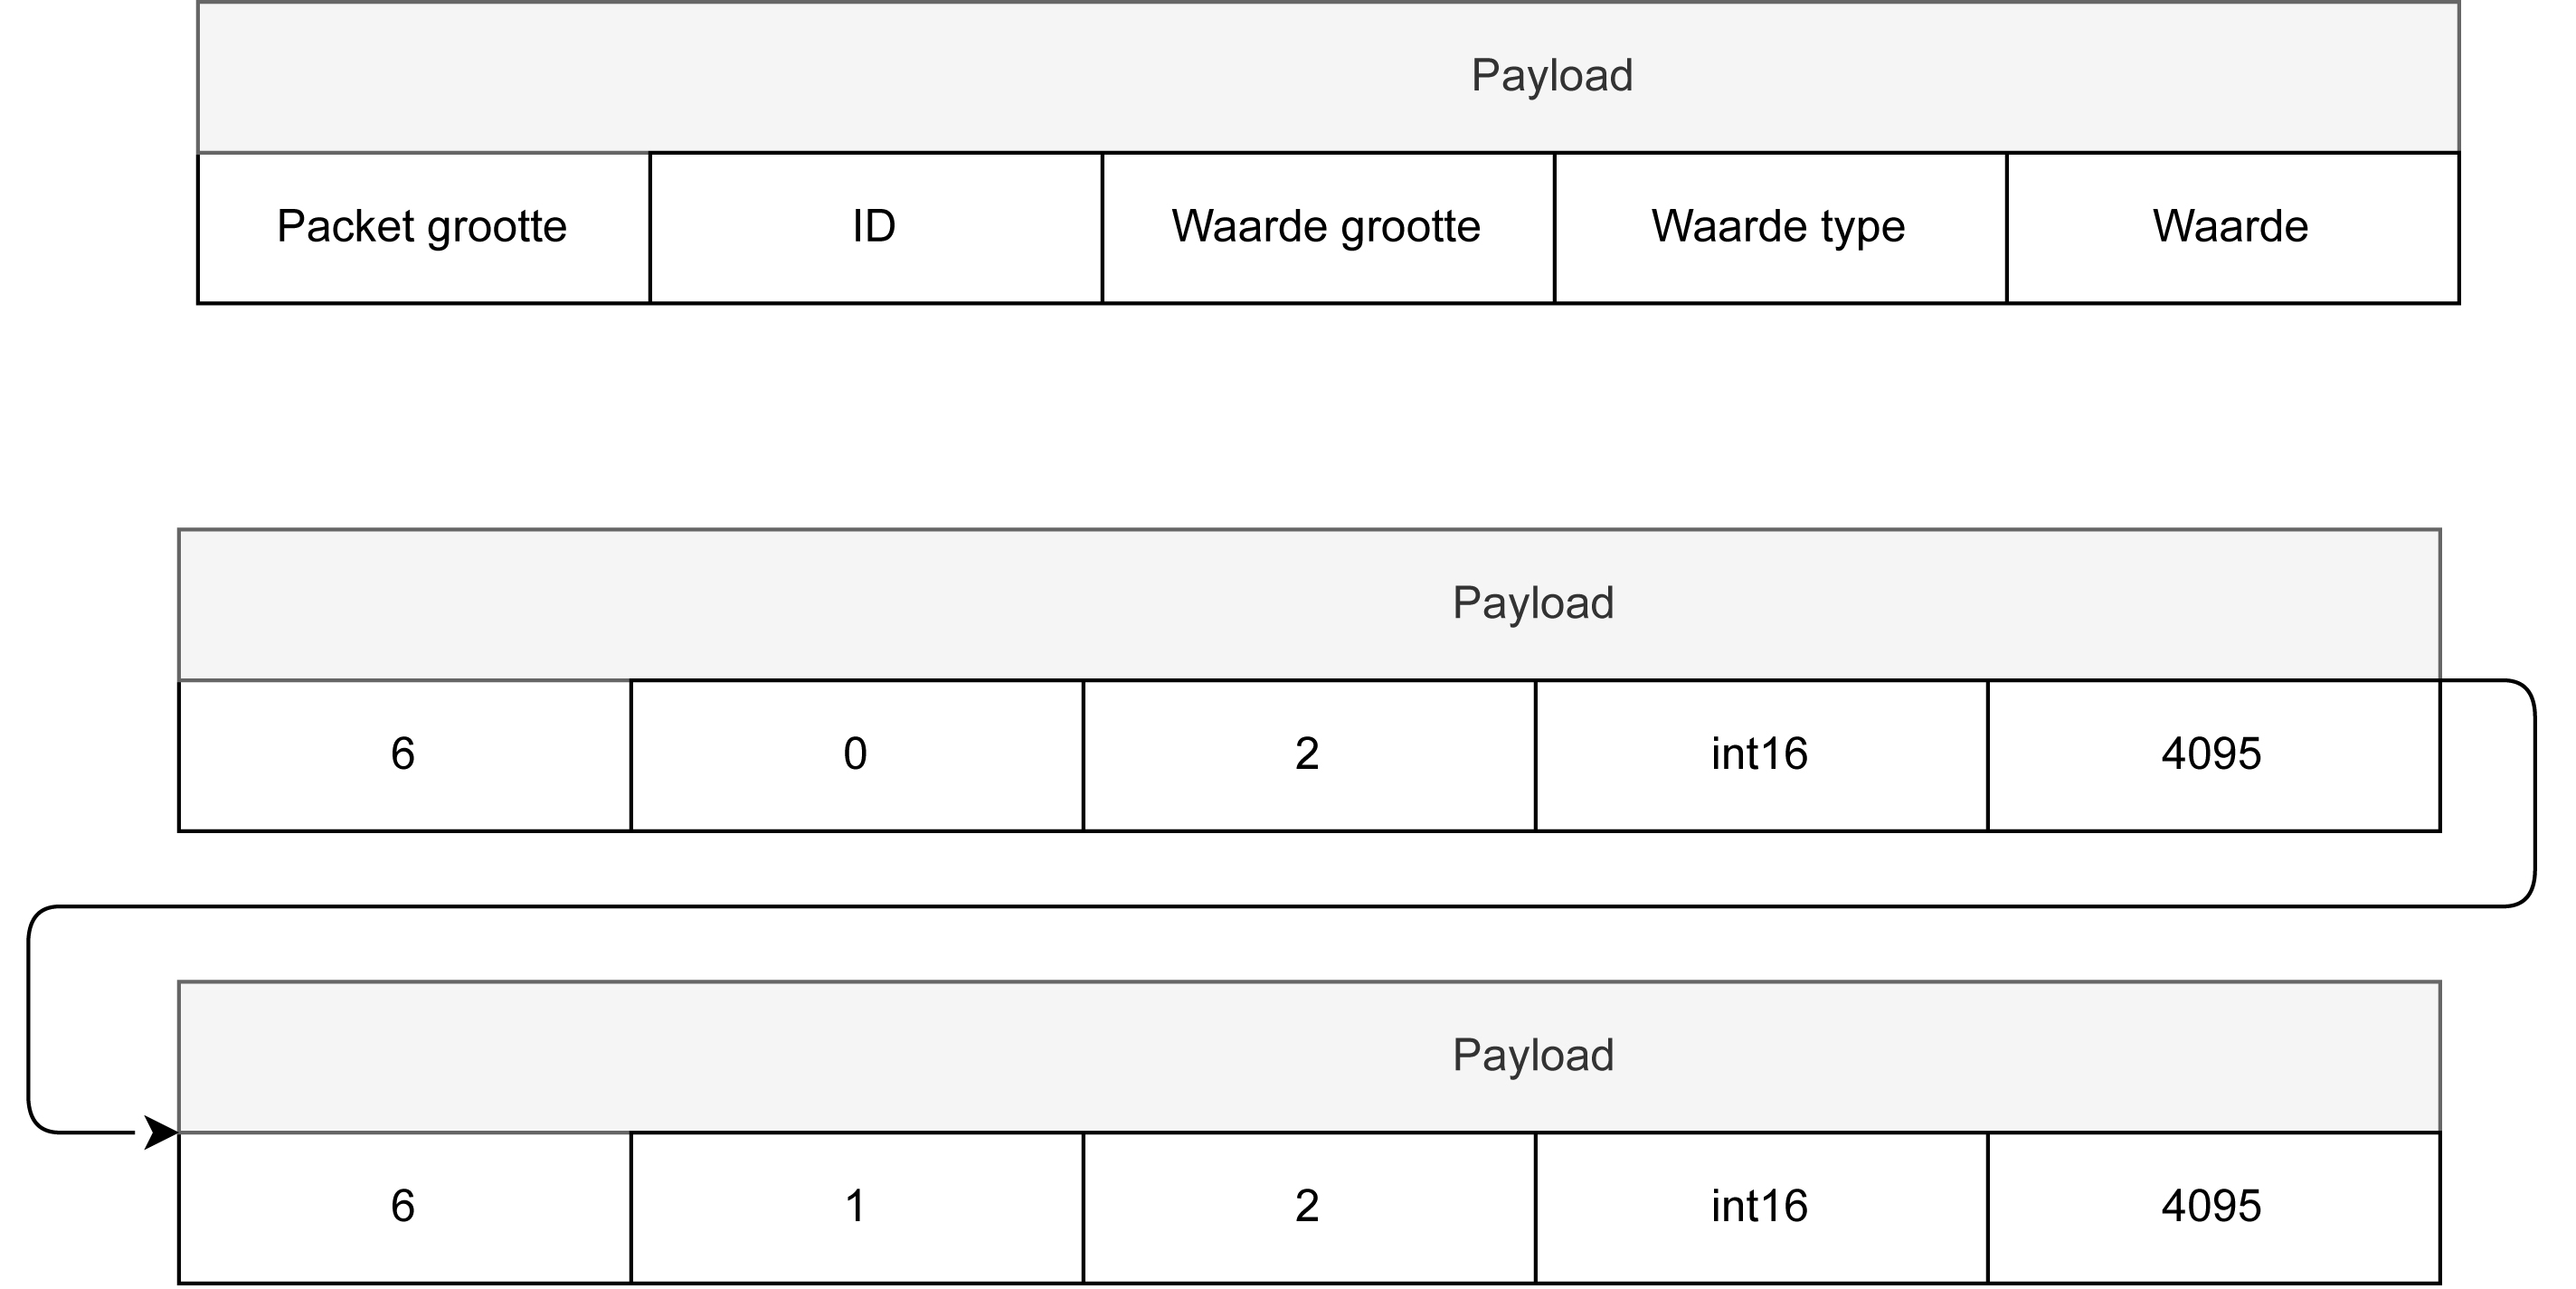
\includegraphics[width=0.75\linewidth]{voorstudie/communicatie/PayloadStructure2-01.jpg}
	\caption{Opbouw en voorbeeld van de payload structuur 2}
\end{figure}

\subsection{Structuur 3}
Dit is de laatste structuur die ontworpen is. Het is een combinatie van structuur 1 en structuur 2. Deze structuur heeft drie onderdelen voor een sensor. Als eerste zal de sensor identificatie meegegeven worden. Daarna komt de waarde grootte in bytes, en uiteindelijk wordt de waarde zelf gegeven. In afbeelding \ref{fig:Structure3} wordt de structuur en een voorbeeld weergeven.
\begin{figure}[h!]
	\label{fig:Structure3}

	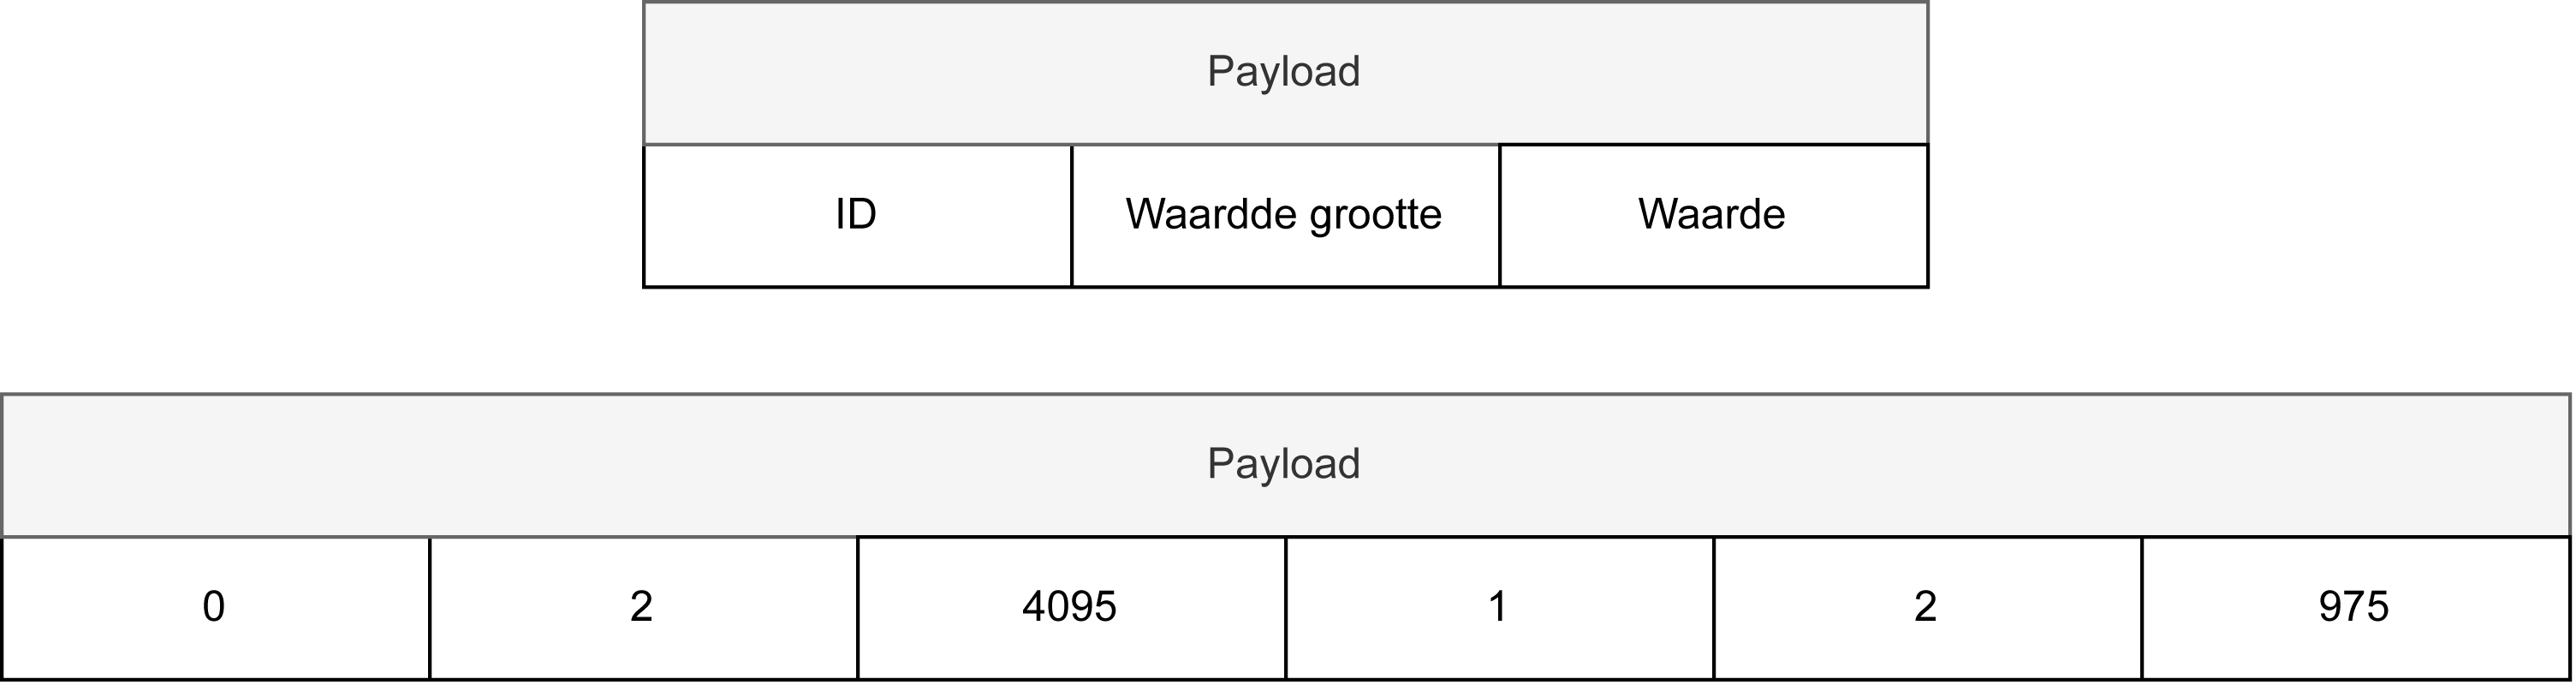
\includegraphics[width=\linewidth]{voorstudie/communicatie/PayloadStructure3-01.jpg}
	\caption{Opbouw en voorbeeld van de payload structuur 3}
\end{figure}

\newpage
\subsection{Communicatie flow}
Hieronder is in in figuur \ref{fig:comflow} te zien hoe de communicatie via CAN-bus gedaan wordt als er een bericht ontvangen wordt van het eindsysteem. Om een connectie te creëren zijn een aantal stappen nodig om dit goed af te handelen. Het hoofdsysteem kan verschillende type berichten sturen, in het vorige hoofdstuk is er vooral gefocust op de sensor payload structuur. Maar voor elk type bericht zal het apart afgehandeld worden. Er wordt dus eerst gecheckt wat voor type bericht het is, en daarvan splits het op in twee sectoren. De linker sector is een simpele structuur waarbij alleen wat data opgehaald of een karakter meegegeven moet worden. Bij de rechter sector wordt de payload structuur opgezet als eerste voor elke sensor dat de Satellite heeft. Dan wordt de payload berekend in bytes. Met de grootte in bytes kan het packet gemaakt worden. Vervolgens wordt het opgestuurd, dit zal een status code teruggeven. Als de communicatie al bezig is met iets versturen zal hierop gewacht moeten worden. Bij andere errors, failures zal een rood lichtje branden als status.
\begin{figure}[h!]
	\centering
	\label{fig:comflow}

	\includegraphics[width=0.7\linewidth]{ontwerp/communicatie/DataFlow.jpg}
	\caption{Activity diagram van de communicatie}
\end{figure}

\newpage
\subsection{Conclusie}
In dit subhoofdstuk is gekeken naar een manier om de huidige CAN Bus protocol zo aan te passen zodat het beter aansluit op de Satellite. De Satellite heeft verschillende sensoren die allemaal uiteindelijk in een payload moeten komen. Omdat het hoofdsysteem niet weet wat voor sensoren de Satellite op enig moment heeft, betekent het dat dit problemen kan veroorzaken. De nieuwe structuur voor de payload moet simpel te implementeren zijn, maar de payload moet ook niet veel groter worden. De eerste structuur is het simpelste maar is lastiger om te implementeren. Het grootste probleem is dat de buffer niet weet waar de volgende sensor begint. De waarde van sensor kan bijvoorbeeld 2 bytes zijn of 8 bytes. Het voordeel van structuur 1 is dat het een kleine structuur is waardoor de totale hoeveelheid data die opgestuurd wordt niet veel groter wordt. Structuur 2 is het tegenovergestelde van structuur 1, structuur 2 is makkelijk te implementeren omdat precies gezien kan worden wat verwacht kan worden per byte. Het probleem van structuur 2 is dat het veel groter is in bytes. Uiteindelijk is er nog structuur 3 en die zit tussen structuur 1 en 2, in vergelijking met hoe simpel het is om te implementeren en packet grootte. Een samenvatting van de structuren is te vinden in tabel \ref{tab:samenvattingstructuur}. \newline

\begin{table}[h!]
	\centering
	\caption{Samenvatting van CAN Payload structuren}
	\label{tab:samenvattingstructuur}
	\begin{tabular}{lll}
	\toprule
		Structuur nummer & Implementatie moeilijkheid & Packet grootte             \\ \midrule
		1                & Lastig                     & Klein (2 tot 9 bytes)      \\
		2                & Simpel                     & Groot (5 tot 12 bytes)     \\
		3                & Simpel                     & Gemiddeld (3 tot 10 bytes) \\ \bottomrule
	\end{tabular}%
\end{table}

\noindent In dit subhoofdstuk is er gekeken naar de volgende deelvraag \textbf{Hoe kan er een robuuste communicatie gecreëerd worden tussen het hoofdsysteem en Satellite?} Er is gekeken naar de moeilijkheid van de implementatie en de grootte van de payload. Deze twee onderdelen spelen een belangrijk onderdeel bij een robuuste communicatie. Daarom is er gekozen voor structuur 3, dit is een vrij simpele implementatie, en vergroot de payload maar weinig. Met deze payload-structuur weet het hoofdsysteem precies wat er gaat komen en hoeveel sensoren aan de Satellite verbonden zijn.
\newpage

\newpage
\section{Validatie}
Elke nieuwe hardware wat aan Satellite wordt geleverd zal door Sensor Maritime moeten gevalideerd moeten worden. Er zal als eerst beschreven worden welke porten er getest worden. De volgende type porten worden besproken. Ten eerste zal er gekeken worden naar DIP schakelaars, digitale output, analoge input, relay en uiteindelijk seriele communicatie. \newline

\noindent De Satellite heeft verschilllende porten porten zijn die gebruikt kan worden. Elke type port wordt beschreven in de volgende hoofdstukken. In deze hoofdstukken wordt beschreven wat de port moet doen en hoe dit getest gaat worden en uiteindelijk wat het verwachte resultaat is.

\subsection{DIP switch}
Een DIP switch bestaat uit een aantal schakelaars die je kan of uit kan zitten \autocite{DIP}. Op de Satellite is er een DIP switch aan bord, die acht schakelaar is heeft. Zeven van de acht worden op het moment gebruikt. Het volgende tabel \ref{tab:hw_val_dip} geeft aan wat de acties zijn als je de schakelaar aan of uit zet. De eerste drie van de schakelaars worden gebruikt als configuratie voor andere porten die worden beschreven in hoofdstuk \ref{Analog Input Signaal}. De laatste vier schakelaars zetten een specifiek pin van de microcontroller hoog of laag.
\begin{table}[h!]
	\caption{DIP switch porten die gevalideerd moeten worden}
	\begin{tabular}{llllp{10cm}}
	\toprule
	\textbf{Naam} & \textbf{GPIO} & \textbf{Pin} & \textbf{IO} & \textbf{Beschrijving}	\\ \toprule
	PU1		& -			& - 	& -    		& Verandert de analog input 1 voltage tussen 0 en 24V	\\
	-		& -			& - 	& -    		& Wordt niet gebruikt.								\\
	PU2		& -			& - 	& -    		& Verandert de analog input 2 voltage tussen 0 en 24V	\\
	PU3		& -			& - 	& -    		& Verandert de analog input 3 voltage tussen 0 en 24V	\\
	ADD0 	& 3			& 10	& Input		& Zet de pin hoog of laag, aan de hand van of het aan staat of niet.		\\
	ADD1 	& 3			& 11	& Input		& Zet de pin hoog of laag, aan de hand van of het aan staat of niet.		\\
	ADD2 	& 3			& 12	& Input		& Zet de pin hoog of laag, aan de hand van of het aan staat of niet.		\\
	ADD3 	& 3			& 0 	& Input		& Zet de pin hoog of laag, aan de hand van of het aan staat of niet.		\\ \bottomrule
	\end{tabular}
	\label{tab:hw_val_dip}
\end{table}

\subsection{Digital output signaal}
De digitale output signaal kan alleen hoog of uit gezet worden, dit betekent dat het geen input modus heeft. De Satellite heeft vier digitale output porten die op 24V of 0V gezet kan worden. Het volgende tabel geeft een overzicht \ref{tab:hw_val_dio}.
\begin{table}[h!]
	\caption{Digital output signalen die gevalideerd moeten worden}
	\begin{tabular}{llllp{10cm}}
	\toprule
	\textbf{Naam} & \textbf{GPIO} & \textbf{Pin} & \textbf{IO} & \textbf{Beschrijving}				 	\\ \toprule
	D1			& 1			& 6    	& Output	& Digital output signaal, op deze pin komt 24V of 0V. \\
	D2			& 1			& 7    	& Output	& Digital output signaal, op deze pin komt 24V of 0V. \\
	D3			& 3			& 3    	& Output	& Digital output signaal, op deze pin komt 24V of 0V. \\
	D4			& 3			& 2   	& Output	& Digital output signaal, op deze pin komt 24V of 0V. \\ \bottomrule
	\end{tabular}
	\label{tab:hw_val_dio}
\end{table}

\subsection{Analog input signaal} \label{Analog Input Signaal}
De analog signalen kan alleen uitgelezen worden, dit betekent dat het alleen een input modus heeft. De Satellite heeft drie analoge input porten aan bord. In het volgende tabel wordt een overzicht gegeven \ref{tab:hw_val_ai}.
\begin{table}[h!]
	\caption{Analog input signalen die gevalideerd moeten worden}
	\begin{tabular}{llllp{9cm}}
	\toprule
	\textbf{IO} & \textbf{GPIO} & \textbf{Pin} & \textbf{Input/Output} & \textbf{Beschrijving}			\\ \toprule
	AI1			& 14		& 2    	& Input		& Analoge input signaal van 0 tot 24 volt.					\\
	AI2			& 14		& 3    	& Input		& Analoge input signaal van 0 tot 24 volt.					\\
	AI3			& 14		& 12   	& Input		& Analoge input signaal van 0 tot 24 volt.					\\  \bottomrule
	\end{tabular}
	\label{tab:hw_val_ai}
\end{table}

\subsection{Relay}
Er is een relay verbonden aan de microcontroller. Een relay is een mechanisch apparaat dat een elektrische connectie maakt tussen twee of meer punten op reactie van de microcontroller. Als er 3,3 volt op de relay gezet wordt zal de relay sluiten en bij 0 volt zal het weer openen gaan. Omdat het mechanisch is moet je dit ook kunnen horen \autocite{relay}. Hieronder is een overzicht van de relay \ref{tab:hw_val_relay}.

\begin{table}[h!]
	\caption{Relay signaal die gevalideerd moeten worden}
	\begin{tabular}{llllp{9cm}}
	\toprule
	\textbf{IO} & \textbf{GPIO} & \textbf{Pin} & \textbf{Input/Output} & \textbf{Beschrijving}			\\ \toprule
	Relay		& 3 & 1   	& Output		& Een mechanische apparaat was dicht of opengaat aan de hand of er 3,3 volt of niet op staat.	\\ \bottomrule
	\end{tabular}
	\label{tab:hw_val_relay}
\end{table}

\subsection{Serieel Communicatie}
De Satellite heeft verschillende porten voor seriele communicatie aanbord. De seriele communicatie middelen zullen gebruikt worden voor communicatie met een eindsysteem of sensoren. Sommige sensoren die Sensor Maritime gebruiken sturen de gegevens via seriele communicatie over. Omdat het zoveel functionaliteiten heeft zal dit grondig getest moeten worden. Satellite heeft verschillende varianten van seriele communicatie, ten eerste zijn er twee UART verbindingen, een RS232 verbinding, en uiteindelijk een RS422 communicatie lijn. \newline

\noindent UART staat voor Universal asynchronous receiver-transmitter. UART stuurt asynchroon data over dit betekent dat er geen klok signaal is die data synchroon maakt. UART wordt universeel genoemd omdat het geconfigureerd om verschillende seriele protocollen te ondersteunen. In plaats van een klok signaal wordt er gebruikt gemaakt van een start bit en een stop bit. Data wordt verstuurd via UART via de gebruiker gespecificeerd frequentie, dit wordt ook wel baudrate genoemd, baudrate wordt gespecificeerd als in bits per seconden (bps) \autocite{UART}. \newline

\noindent RS-232 is anders opgebouwd dan UART. RS-232 is een standaard gedefineerd signaal tussen twee apparaten, waar de signaal naam, doel, spanningniveau en pinnen zijn gedefineerd zijn. Een belangrijk verschil tussen RS-232 en UART is dat de spanningniveau hoger en negatief kan zijn. Het voltage bereik van RS-232 gaat -12 volt tot 12 volt \autocite{RS232}. \newline

\noindent RS-422 is weer een andere vorm van seriele communicatie en heeft kenmerken van RS-232. Het verschil tussen RS-232 en RS-422 is dat het voor de communicatie vier lijnen gebruikt (RX-, RX+, TX+, TX-). Met de vier communicatielijnen kan er full duplex gecommuniceerd worden. Full duplex communicatie betekent dat er twee of meer apparaten in beide richting kan communiceren (ontvangen en verzenden op hetzelfde moment) \autocite{FullDuplex}. RS-232 heeft half-duplex dit houdt in dat via RS-232 alleen handeling gedaan kan worden, bijvoorbeeld eerst ontvangen en dan pas verzenden. \autocite{RS422}.

\noindent In het volgende tabel \ref{tab:hw_val_serieel}wordt een overzicht gegeven van de seriele communicatie die verbonden zijn op de microcontroller. Voor de RS-422 communicatie is alleen twee communicatielijnen aangegeven, omdat dit zo verbonden is op de microcontroller. De Rx+, RX- en TX+, TX- lijnen worden samengevoegd door een chip en dan verbonden naar de microcontroller.
\begin{table}[h!]
	\caption{Seriele communicatie porten die gevalideerd moeten worden}
	\begin{tabular}{llllp{9cm}}
	\toprule
	\textbf{IO} & \textbf{GPIO} & \textbf{Pin} & \textbf{Input/Output} & \textbf{Beschrijving}	\\ \toprule
	UART RX		& 5			& 0    	& Input		& Seriele communicatie ontvangst lijn.			\\
	UART TX		& 5			& 1    	& Output	& Seriele communicatie versturen lijn.			\\
	RS-232 RX	& 3			& 7    	& Input		& Seriele communicatie ontvangst lijn.			\\
	RS-232 TX	& 3			& 8    	& Output	& Seriele communicatie versturen lijn.			\\
	RS-422 RX	& 6			& 3    	& Input		& Seriele communicatie ontvangst lijn.			\\
	RS-422 TX	& 3			& 13   	& Output	& Seriele communicatie versturen lijn.			\\
	UART 2 RX	& 4			& 6    	& Input		& Seriele communicatie ontvangst lijn.			\\
	UART 2 TX	& 4			& 7   	& Output	& Seriele communicatie versturen lijn.			\\ \bottomrule
	\end{tabular}
	\label{tab:hw_val_serieel}
\end{table}

\newpage
\section{Klasse diagram}
Hieronder is een klasse diagram gegeven van de hele applicatie \ref{fig:klassediagram}. Hier zijn een paar onderdelen goed te zien ten eerste, is te zien dat alle sensoren een abstractie laag hebben, die specifieke gekoppeld is aan een sensor  driver. De hardware abstractie lagen die door DAVE zijn gemaakt zijn worden niet getoond in de klasse diagram aangezien dit een externe library is.
\begin{figure}[h!]
	\centering
	\label{fig:klassediagram}
	\caption{Algemene structuur van de applicatie}
	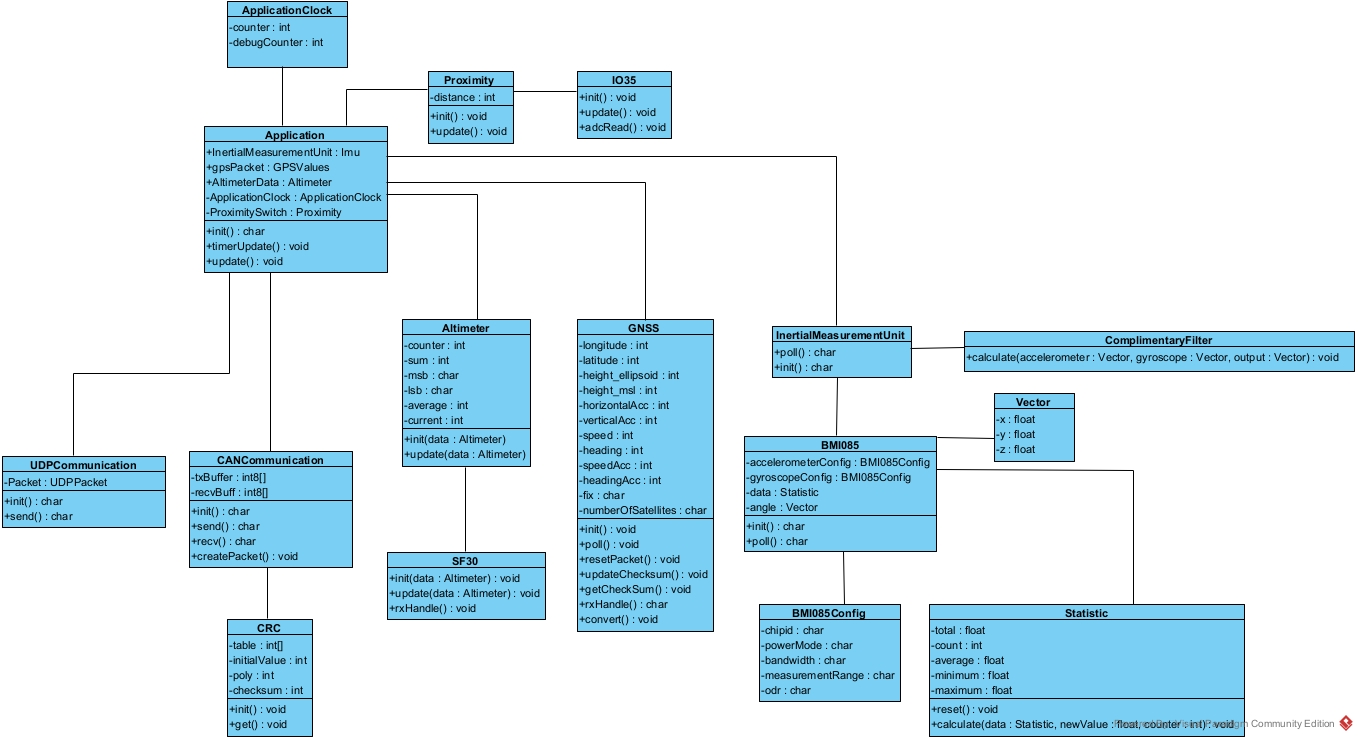
\includegraphics[width=\linewidth]{ontwerp/applicatie/Satellite.jpg}
\end{figure}

	\chapter{Uitvoering NOT DONE}
In dit hoofdstuk wordt de uitvoering en het process beschreven van het afstudeeropdracht. Het project kan opgesplitst worden in een paar grote onderdelen. De uitvoering zal dan ook opgesplitst worden in de volgende fases. Ten eerste wordt er gekeken naar structuur, interfacing, communicatie, sensoren en uiteindelijk transformatie/filters. In deze volgorde is dan ook de applicatie ontwikkeld.

\section{Overzicht}
Om een beeld te krijgen wat er gedaan is in de laatste 20 weken tijdens het afstuderen is er een overzicht gemaakt van welke grootte taken er ontwikkeld zijn. Het diagram laat zien wat er ontwikkeld/ontworpen is en welke stappen hij daarvoor genomen heeft om deze taak goed af te ronden. Er zijn hiervoor een paar fases type gekozen, ten eerste zal er gekeken worden naar het ontwerp, interface, sensor data en communicatie.

\begin{table}[h!]
	\centering
	\caption{Fases van de uitvoering}
	\label{tab:UitvoeringOverzicht}
	\begin{tabular}{lp{13cm}}
	\toprule
	\textbf{Fase} & \textbf{Samenvatting} \\ \midrule
	Ontwerp & In deze fase is onderzoek gedaan naar generiek software ontwerp en de payload structuur voor de CAN communicatie. Daarnaast is er ook gekeken naar het hardware validatie. \\
	Interface & In de interface fase is er test en debug applicatie ontworpen voor de applicatie en de hardwarevalidatie onderdeel. \\
	Communicatie & Hier wordt er gekeken naar de UDP communicatie en CAN BUS communicatie.                      \\
	Sensors  & Hier wordt er gekeken hoe er verschillende sensoren uitgelezen kunnen worden via verschillende protocollen.                      \\ 
	Transformatie en filter & In deze fase wordt er gekeken hoe de data geprocesed wordt. \\ \bottomrule
	\end{tabular}
\end{table}

\newpage
\section{Ontwerp}
Het ontwerp van de applicatie is het belangrijkste onderdeel van de applicatie, dit beantwoord namelijk de hoofdvraag en twee deelvragen. Dit moet dan ook goed onderzocht worden, zodat in toekomst Sensor Maritime veel sensoren kan ondersteunen zonder grotere aanpassing aan de applicatie. Dat is het uiteindelijk doel van het ontwerp hoe kan er met minimale verandering aan de applicatie nieuwe sensoren toegevoegd worden. Met het ontwerp kunnen de volgende fases gebouwd worden op basis van het bedachte structuur. Het ontwerp is een groot onderdeel en combinatie van verschillende onderdelen van de applicatie en dit zal dan ook in dit hoofdstuk opgesplitst worden in verschillende onderdelen.

\subsection{Applicatie}
Om het structuur op te zetten moest er gekeken worden naar welke programmeertaal er gebruikt gaat worden. Dit was dan ook de eerste taak die student op zich nam. Omdat dit goed te kiezen moet er een analyses gemaakt worden op, wat gebruikt Sensor Maritime standaard. Daarnaast moet erook gekeken worden bestaan er software ontwerpen/design patterns die een generieke structuur creeëren. De programmeertaal keuze was met de stagebegeleider besproken waarbij, er twee opties onstaan zijn. De twee opties waren C of C++, Sensor Maritime gebruikt standaard voor de embedded producten C. Sensor Maritime had minder ervaring met C++. Met deze informatie is de stagair gaan kijken naar hoe de structuur zou opgebouwd kan worden in zowel C als in C++. Met C++ zal er meer abstractie gemaakt kunnen worden omdat je dan werkt met object georienteerd programmeren. Alleen zullen de bestaande lagen van de applicatie structuur bestaan. De toegevoegde waarden van C++ had niet genoeg impact om het te gebruiken. \newline

\noindent Met de taal gekozen is een software abstractie gemaakt waardoor zo veel mogelijk generiek is. Dit is aan de hand van de applicatie lagen en de preprocessor gedaan. Met de applicatie lagen kan er aanpassingen of toevoegingen gemaakt worden aan de applicatie zonder dat de applicatie logica veranderd hoeft te worden. De preprocessor zorgt er voor dat er gemakkelijk functionaliteiten en sensoren aan of uit gezet kan worden. Met de preprocessor kan er bijvoorbeeld makkelijk gekozen worden welke versie sensor er gebruikt moet worden. De overige sensoren worden dan ook niet mee gecompileerd.

\subsection{CAN}
Het volgende onderdeel van het structuur is de communicatie via de CAN BUS. Hiervoor is al een bestaand protocol die door Sensor Maritime is ontworpen. Het probleem van dit protocol is dat het niet ontwikkeld is voor eindsystemen met verschillende sensoren. Er wordt nu er van uitgegaan dat de payload van het packet, maar een sensor data heeft. Terwijl de Satellite veel meer dan een sensor aanbord kan hebben. Dus het hoofdsysteem die de sensor data wil weet dan niet wat voor sensor data hij ontvangt, is het 1 of 2 sensoren en welke sensoren zijn het dan. Hier moest een systeem bedacht voor worden. Hiervoor zijn drie ontwerpen gemaakt. Een simpel structuur, een generiek modulair structuur en een structuur wat er tussen zit. Dit is voorgelegd bij het stagebedrijf, hierover is gediscussieerd wat het meest optimale structuur is voor zowel het eindsysteem als de Satellite. Uit deze discussie is de structuur gekozen was er tussen in zit.

\subsection{Hardware validatie}
Een van de taken die Sensor Maritime mij heeft opgelegd is om een systeem te bedenken, zodat als Sensor Maritime nieuw Satellite hardware hebben dat ze die makkelijk kunnen testen. De onderdelen die getest moeten worden zijn IO porten de Satellite. Het manier van testen en wat getest moet worden is als eerst besproken met de stagebegeleider. Hiervoor is een testplan ontwikkeld dat voor elke IO port een manier van testen heeft. Aan de hand van de testplan is er een test applicatie geschreven wat de applicatie test aan de hand wat er beschreven is bij het testplan. Om alle firmware die voor de Satellite is ontwikkeld is de Satellite applicatie en test applicatie samengevoegd. Hiervoor is de preprocessor gebruikt. Sensor Maritime hoeft alleen maar een definitie uit of aan te zetten en opnieuw compileren. Hiermee kan Sensor Maritime makkelijk wisselen tussen hardware validatie en echte Satellite applicatie.

\section{Interface}
Om de uiteindelijk Satellite applicatie, en testplan applicatie te kunnen testen zal er een applicatie nodig zijn die kijkt of de hardware applicatie wel werken na toebehoren. Hiervoor zijn twee desktop applicaties gemaakt. Deze twee applicaties zullen opgesplitst worden in subhoofdstukken die hieronder beschreven zijn.

\subsection{Satellite debug applicatie}
De debug applicatie is geschreven om te testen of de functionaliteiten van de applicatie werken. Dit geeft de ontwikkelaar een beeld of de verwachte data kloppend is. De Satellite communiceert met de debug applicatie via UDP, hiervoor is gekozen aangezien de klant het uiteindelijk zo verwacht. De debug applicatie moet dan ook een simulatie zijn van wat de klant verwacht te ontvangen.

\subsection{Testplan applicatie}
De testplan applicatie is ontwikkeld om sommige onderdelen van de testplan te testen. Serieele communicatie is lastig om te verifiëren zonder een desktop applicatie. Het doel van de testplan applicatie is dat Sensor Maritime snel kan zien of de hardware werkt zoals verwacht.

\section{Communicatie}
Het communicatie is een groot onderdeel van de applicatie. Vanuit Satellite moet er gecommuniceerd worden met een eindsysteem. Tijdens de implementatie van de applicatie zijn verschillende vormen van communicatie gebruikt met het eindsysteem. Deze twee vormen van communicatie zijn bepaald door de klant. \newline

\noindent De eerste vorm van communicatie die ontwikkeld is de UDP. Via UDP communicatie wordt verschillende sensor data opgestuurd om de seconden. Voor elke sensor wordt een apart packet opgestuurd hiervoor is een standaard structuur voor bedacht. Ten eerste wordt alle data opgestuurd in bytes. vervolgens wordt er een prefix toegevoegd met maximaal acht bytes, bijvoorbeeld \textit{imu,}. Met deze prefix weet het eindsysteem wat voor data ontvangen kan worden. Vervolgens wordt er een sensor speciek payload opgestuurd. De payload structuur is gespecifeerd met de klant en is per sensor verschillend. \newline

\noindent De twee vorm van communicatie gaat via CAN BUS. Dit wordt alleen gebruikt om te kunnen communiceren met het hoofdsysteem. Het hoofdsysteem kan verschillende dingen vragen aan de Satellite en dit moet allemaal afgehandeld worden. Bijvoorbeeld het hoofdsysteem kan de status opvragen van de Satellite. Zodra de Satellite dit ontvangt moet het ontvangen packet opgebouwd worden en gecheckt zijn of het ontvangen packet ook echt is wat er opgestuurd is door het hoofdsysteem. Als dat gedaan moet er gekeken worden wat vraagt het hoofdsysteem aan de Satellite. Hiervoor zijn verschillende states gemaakt die op elke type bericht een antwoord kan geven. Dus als de hoofdsysteem de status opvraagt van de Satellite zal de Satellite zijn status terugsturen.


\section{Sensors}
De volgende fase was om voor de sensoren een abstractie en driver laag ontwikkelen. De abstractie laag zal bepalen hoe de sensor zich moet gedragen. De abstractie laag is het tussenpersoon van de applicatie logica en sensor drivers. Het idee is dan ook dat de abstractie laag met de hulp van preprocessor bepaald welke sensor gebruikt gaat worden. Voor elke sensor is een nieuwe definitie toegevoegd wat bepaald of de sensor abstractie laag de sensor driver aanroept of niet. Er zijn verschillende type sensoren, sommige sensoren werken via SPI, serieel of juist analoog. Dit wordt allemaal uitgewerkt in de sensor driver. Elke sensor is anders in werking, dus drivers zal altijd toegevoegd worden.

\section{Transformatie en filters}
Dit onderdeel gebeurt nadat de sensor data is opgehaald. Bepaalde data moet verwerkt worden, zodat de klant iets heeft aan de data die laten zien wordt. Op het moment wordt er maar op een sensor deze transformatie/filter toegevoegd, dit is op inertial measurement unit (imu). De imu bestaat uit twee onderdelen, ten eerste is een versnellingsmeter aan boord. De Versnellingsmeter meet de versnelling in de x, y en z axis. Daarnaast bezit de imu ook een gyroscoop wat de hoekversnelling per seconde geeft. Met de imu kan je ook de hoek berekenen, de componenten los hebben beide problemen. De versnellingsmeter heeft veel ruis en kan af en toe verspringen. De gyroscoop is alleen accuraat in het begin, naar mate de tijd vordert zal de waarde langzaam wegdriften. Los zijn de componenten niet goed genoeg om een accurate hoekmeting te krijgen, maar als beide componenten samengevoegd wordt los je beide problemen op. Om de twee componenten samen te voegen zal er gebruikt gemaakt worden van een filter. Hiervoor is de complimentary filter gebruikt. De complimentary filter zegt dat je een percentage van de gyroscoop en een percentage van de versnellingsmeter moet nemen, dit moet samen 100\% zijn. De wiskundige notatie gaat als volgt \ref{eqn:compfilter}, hierbij worden een aantal variable gebruikt. De eerste variable is $\alpha$, dit geeft aan hoeveel procent je van de gyroscoop wil, in de huidige implementatie is hiervoor $0,02$ gebruikt. Dit betekent dat er $98\%$ gebruikt wordt van de gyroscoop en $2\%$ van de versnellingsmeter. Vervolgens wordt de vorige hoek gepakt en dit wordt toegevoegd aan de huidige gyroscoop waarden wat vervolgens vermenigvuldigd wordt door de frequency. Uiteindelijk wordt de versnellingsmeter toegevoegd.

\begin{equation}
\label{eqn:compfilter}
	\begin{array}{l}
	roll[t] = (1 - \alpha) * (roll[t - 1] + G_{x} * \Delta t) + \alpha * A_{roll} \\
	pitch[t] = (1 - \alpha) * (pitch[t - 1] + G_{y} * \Delta t) + \alpha * A_{pitch} \\ 
	yaw[t] = (1 - \alpha) * (yaw[t - 1] + G_{z} * \Delta t) + \alpha * A_{yaw} 
\end{array}
\end{equation}
	\chapter{Testen}
In dit hoofdstuk wordt er gekeken naar de testen die gedaan is tijdens het traject, ten eerste wordt er gekeken naar de hardware validatie testplan, maar ook het testplan voor de applicatie. Testen in softwareontwikkeling is een belangrijk onderdeel, hiermee kan er goed gekeken hoe robuust de applicatie is geworden.

\section{Testplan hardware validatie} \label{sec:hwtestplan}
Dit is het testplan die bedacht is om de alle porten van de Satellite te testen, dit is testplan die wordt gebruikt bij Satellite hardware. Hiermee kan Sensor Maritime heel snel de hardware verifiëren.
\subsection{DIP switch}
De eerste drie schakelaars worden anders getest in vergelijking met de laatste vier. De laatste vier schakelaars maken vier leds branden die op Satellite zitten. In de volgende tabel \ref{tab:hw_val_dip_testplan} is een overzicht van het testplan:
\begin{table}[h!]
	\caption{DIP switch porten testplan}
	\begin{tabular}{lp{14.5cm}}
	\toprule
	\textbf{Naam} 	& \textbf{Verwachte resultaat} \\ \toprule
	PU1				& Als het aan gezet wordt de range van de analoge input 1 verhoogt naar 24 volt, dit verhoogt de waarde wat de microcontroller leest, de waarde wordt laten zien op een GUI.\\
	-				& Wordt niet getest. \\
	PU2				& Als het aan gezet wordt de range van de analoge input 2 verhoogt naar 24 volt, dit verhoogt de waarde wat de microcontroller leest, de waarde wordt laten zien op een GUI.\\
	PU3				& Als het aan gezet wordt de range van de analoge input 3 verhoogt  naar 24 volt, dit verhoogt de waarde wat de microcontroller leest, de waarde wordt laten zien op een GUI. \\
	ADD0 			& Zet 3.3V op de pin van de microcontroller, als de microcontroller 3.3V detecteert zet het led 0 aan.\\
	ADD1 			& Zet 3.3V op de pin van de microcontroller, als de microcontroller 3.3V detecteert zet het led 1 aan.\\
	ADD2 			& Zet 3.3V op de pin van de microcontroller, als de microcontroller 3.3V detecteert zet het led 2 aan.\\
	ADD3 			& Zet 3.3V op de pin van de microcontroller, als de microcontroller 3.3V detecteert zet het led 3 aan.\\ \bottomrule
	\end{tabular}
	\label{tab:hw_val_dip_testplan}
\end{table}

\newpage
\subsection{Digital output signaal}
Alle digitale output porten voeren dezelfde actie. Het doel is dat als een LED verbonden is met de port dat die dan aan of uit gaat om de 1 seconden.
\begin{table}[h!]
	\caption{Digital output signalen testplan}
	\begin{tabular}{lp{14.5cm}}
	\toprule
	\textbf{Naam} 	& \textbf{Verwachte resultaat} \\ \toprule
	D1	&	Als op de pin 24V staat gaat het lampje aan, en bij 0V uit gaat het uit. Dit gebeurt om 1 seconden. \\			
	D2	&	Als op de pin 24V staat gaat het lampje aan, en bij 0V uit gaat het uit. Dit gebeurt om 1 seconden. \\			
	D3	&	Als op de pin 24V staat gaat het lampje aan, en bij 0V uit gaat het uit. Dit gebeurt om 1 seconden. \\			
	D4	&	Als op de pin 24V staat gaat het lampje aan, en bij 0V uit gaat het uit. Dit gebeurt om 1 seconden. \\ \bottomrule
	\end{tabular}
	\label{tab:hw_val_dio_testplan}
\end{table}

\subsection{Analog input signaal}
Aan de hand wat is beschreven zal er gebruik gemaakt worden van de DIP schakelaars PU1, PU2, en PU3 om de analoge input te testen. De microcontroller heeft een 12 bit Analog to Digital Converter (ADC) \autocite{microcontroller}. Dit betekent dat het bereik van analoge input porten van 0 tot 4096 ($2^{12}$) is. Dus bij 24 volt zal de microcontroller ongeveer 4096 in lezen, het getal kan af en toe lager zijn in verband met ruis. Bij 0 volt zal de microcontroller 0 in lezen. PU1, PU2, PU3 zet het analoge bereik tussen 3,3 volt en 24 volt. Dit betekent als PU1, PU2 of PU3 uitstaan dat de maximale bereik 3,3 volt is en als het aan staat is de bereik 24 Volt. Om het bereik te testen zal er  gemaakt worden van een Graphical User Interface (GUI). De microcontroller zal om 100 microseconden de analoge input omzetten naar een digitale waarden en dit opsturen over UDP. Hiermee kan geverifieerd worden dat als de DIP schakelaars uitstaan dat het bereik van de waarden van 0 tot 1100 gaan. Als de DIP schakelaars aan staan dan zal het bereik zijn van 0 tot 4096. Hieronder is een overzicht van hoe de analoge input porten gevalideerd worden \ref{tab:hw_val_ai_testplan}.
\begin{table}[h!]
	\caption{Testplan voor de analoge input signalen}
	\begin{tabular}{lp{14.5cm}}
	\toprule
	\textbf{Naam} 	& \textbf{Verwachte resultaat} \\ \toprule
	AI1			& Als de schakelaar PU1 van de schakelaar aangezet wordt dan zal de data bereik op de graphical user interface aangepast worden naar 0 tot 4096. Als het dip schakelaar uit staat dan zal de bereik maar van 0 tot 1100 gaan.\\
	AI2			& Als de schakelaar PU1 van de schakelaar aangezet wordt dan zal de data bereik op de graphical user interface aangepast worden naar 0 tot 4096. Als het dip schakelaar uit staat dan zal de bereik maar van 0 tot 1100 gaan.\\
	AI3			& Als de schakelaar PU1 van de schakelaar aangezet wordt dan zal de data bereik op de graphical user interface aangepast worden naar 0 tot 4096. Als het dip schakelaar uit staat dan zal de bereik maar van 0 tot 1100 gaan.\\  \bottomrule
	\end{tabular}
	\label{tab:hw_val_ai_testplan}
\end{table}

\subsection{Relay}
De relay geeft bij het sluiten en het openen van de mechanische connectie een luid geluid wat op normale afstand van het apparaat te horen moet zijn. Het testplan van de relay wordt dan ook op geluid gedaan. De relay zal dan voor vijf seconden aan gaan, en vervolgens weer voor vijf seconden uitgaan. Hieronder is een overzicht van de relay testplan \ref{tab:hw_val_relay_testplan}.

\begin{table}[h!]
	\caption{Testplan voor de relay}
	\begin{tabular}{lp{14.5cm}}
	\toprule
	\textbf{Naam} 	& \textbf{Verwachte resultaat} \\ \toprule
	Relay			& De microcontroller zet de pin van de relay voor vijf seconden hoog, als dit gebeurt hoor je een klik te horen. Na vijf seconden zal deze pin weer laag gezet worden, dit moet ook gehoord kunnen worden.\\  \bottomrule
	\end{tabular}
	\label{tab:hw_val_relay_testplan}
\end{table}


\subsection{Serieel communicatie}
Om de serieel communicatie te testen wordt er gebruik gemaakt van GUI. Deze GUI vraagt de om gebruikers input hierin kan de gebruiker een tekst schrijven en dit wordt opgestuurd. De tekst heeft een limiet van maximaal 32 karakters. Er zal hier automatisch een newline karakter toegevoegd worden zodat de microcontroller weet dat dit het einde van het gebruikers bericht is. Het bericht wordt opgestuurd naar de microcontroller en zal de data verwerken. De microcontroller zal dan een antwoord geven als volgt, ten eerste zal de microcontroller vertellen welke variant van communicatie is gebruikt en daarna zal het toevoegen wat de microcontroller ontvangen heeft van de gebruiker. Hieronder is een overzicht \ref{fig:testplanserieel} van hoe het testplan zal werken.

\begin{figure}[h!]
	\centering

	\label{fig:testplanserieel}
	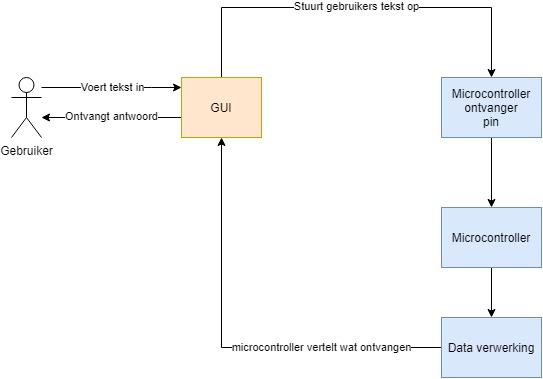
\includegraphics[width=0.5\linewidth]{voorstudie/testplan/Serieel.jpg}
	\caption{Testplan serieel communicatie}
\end{figure}

\newpage

\subsection{GUI}
\section{Applicatie}
De applicatie moet voldoen aan de eisen en doelstelling die bepaald zijn in hoofdstuk \ref{ch:aanpak}, hiervoor is gebruikt gemaakt van twee manieren van testen. Ten eerste wordt er gebruikt gemaakt van een GUI die data ontvangt van de Satellite en toont op GUI in vorm van grafieken en tabellen. Er is hiervoor een nieuw project begonnen die stagiair zelf ontwikkeld heeft. De tweede manier van testen is gebruikt maken van de onboard LED's die de Satellite standaard beschikt. De Satellite heeft in totaal vier LED's die softwareontwikkelaar aan of uit kan zetten. 



\subsection{GUI}
Om de applicatie te testen is er gebruik gemaakt van een desktopapplicatie die alle data ontvangt en visualiseert in verschillende grafieken. Dit geeft de gebruiker direct input of een applicatie werkt na toebehoren. Er is voor elke sensor een nieuw tabblad gemaakt waarop dat weergeeft wordt. Om de applicatie goed te testen is dan ook de applicatie gebruikt op lange termijn zodat de softwareontwikkelaar ook weet of het over drie uur nog steeds zal werken. Hieronder is een voorbeeld \ref{fig:guitest} hoe de user interface eruitziet. 
\begin{figure}[h!]
	\centering

	\label{fig:guitest}
	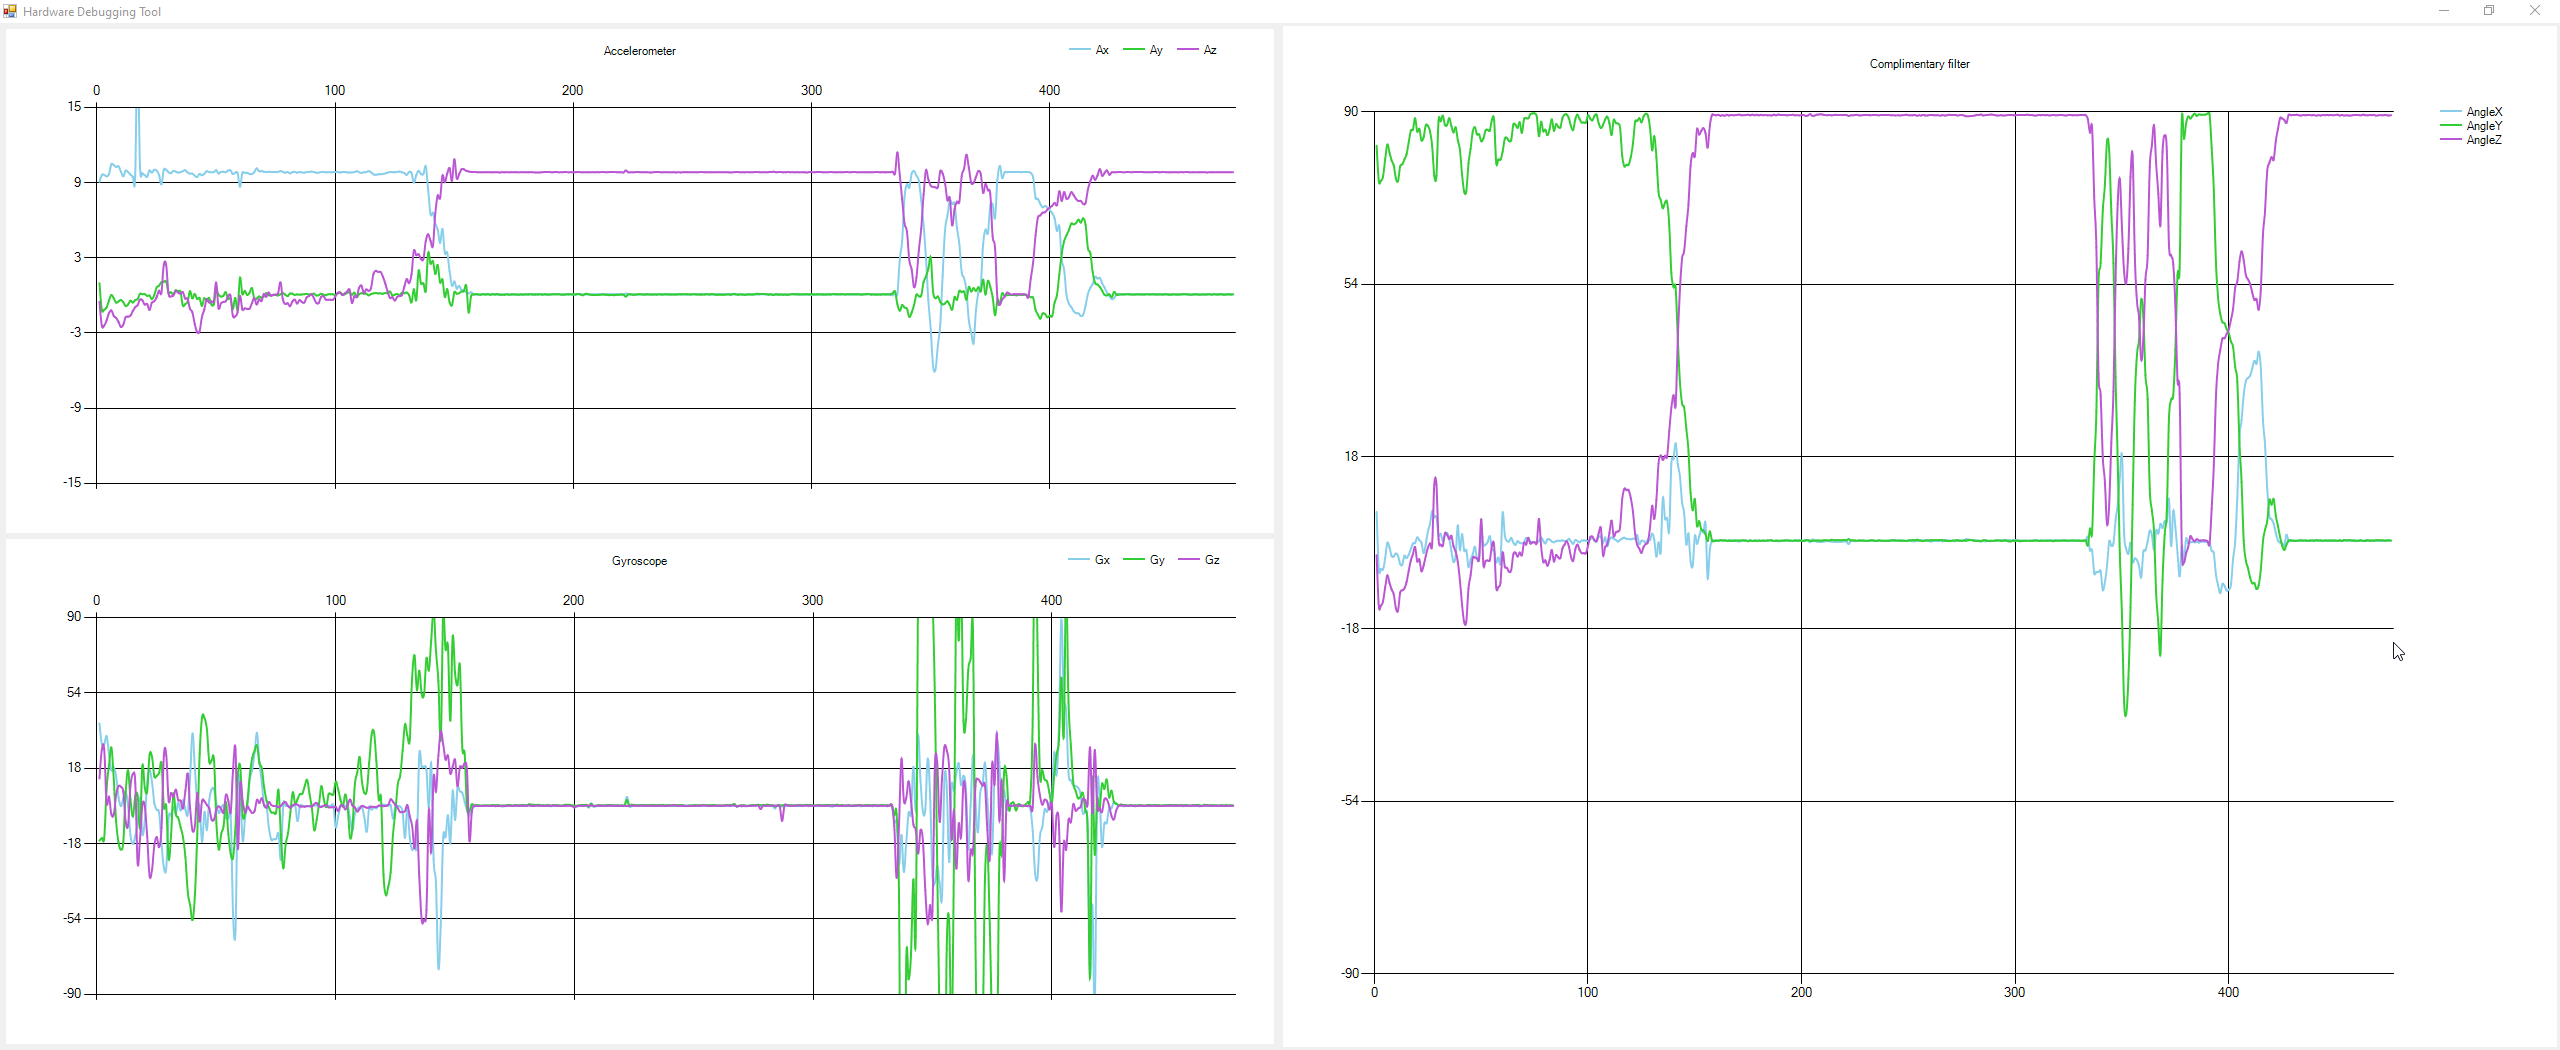
\includegraphics[width=\linewidth]{testen/GUI.png}
	\caption{Desktopapplicatie om Satellite te testen}
\end{figure}

\newpage
\subsection{LED's}
Er zitten standaard vier LED’s op het boordje, en alle vier hebben een ander kleur. De LED’s zijn puur voor de softwareontwikkelaar en zal door de kapitein van een binnenvaartschip niet gezien worden. Hieronder is gedefinieerd wanneer de LED’s gebruikt worden en waarvoor ze gebruikt worden \ref{tab:leds}. Er is voor errors en warnings de standaardkleuren rood en geel gebruikt. Daarnaast wordt ervoor het data ophalen een groen LED laten zien als dit succesvol is gedaan, bij fouten van het ophalen van de sensor data wordt een geel of rood LED getoond. Dit is gebaseerd hoe fout het is gegaan. Bij het versturen van sensor data of bij het ontvangen van data wordt er een blauw licht vertoont.
\begin{table}[h!]
	\caption{Satellite onboard LED beschrijving}
	\begin{tabular}{lp{14.5cm}}
	\toprule
	\textbf{LED Kleur} 	& \textbf{Beschrijving} \\ \toprule
	Groen	& Er wordt sensor data opgehaald\\
	Rood	& Error \\
	Blauw	& Data wordt opgestuurd, of data is ontvangen \\
	Geel	& Er is iets fout gegaan, Satellite probeert het op te lossen\\  \bottomrule
	\end{tabular}
	\label{tab:leds}
\end{table}
	\chapter{Resultaat}
In dit hoofdstuk zullen alle resultaten van de afstudeeropdracht beschreven worden. De resultaten zullen opgesplitst zijn in twee onderdelen. Ten eerste zal er teruggekoppeld worden op de doelstellingen en eisen. Ten tweede zal er gekeken worden of de Satellite voldoet aan het opgezette hardware testplan.

\section{Doelstellingen}
In het begin van het project zijn er drie doelstellingen gedefineerd, de doelstellingen hebben als taak om een overzicht te krijgen wat er precies bereikt zal moeten worden. De volgende doelstellingen zijn hieronder gedefineerd. De doelstellingen kunnen opgesplitst worden in twee onderdelen, het eerste onderdeel is hardwarevalidatie. Het tweede onderdeel focust zich op het onderdeel om een generieke applicatie en robuuste communicatie te ontwikkelen. In de volgende subhoofdstukken zal er gekeken worden per onderdeel wat het resultaat van de doelstelling is.
\begin{enumerate}
	\item De Satellite IO porten zijn volledig getest, en kunnen communiceren met sensoren.
	\item De Satellite heeft een robuuste communicatie over CAN en UDP.
	\item Generiek en modulair opgebouwde software, waardoor het in de toekomst makkelijk uitgebreid kan worden.
\end{enumerate}

\subsection{Hardware validatie}
Vanuit Sensor Maritime is er gevraagd om een manier te ontwikkelen om snel nieuwe hardware van de Satellite te kunnen testen. Hiervoor is een testplan ontwikkeld dat alle porten test. In dit testplan is beschreven welke porten getest wordt, wat de verwachting is en hoe het is aangesloten aan de microcontroller. Het testplan is opgesplitst in type porten. De Satellite heeft vijf verschillende porten, de porten zijn een DIP switch, digitaal output signaal, analoog input signaal, relay, en seriële porten. Voor elke type port is een aparte manier van testen bedacht. \newline

\noindent De hardwarevalidatie heeft ook een implementatie nodig, ten eerste moet er software geschreven worden voor de Satellite, en voor de desktop. De Satellite voert de handelingen uit zoals die beschreven zijn in het testplan, en de desktopapplicatie visualiseert. Het is nu zo opgebouwd dat de Satellite de resultaten van het testplan opstuurt naar de applicatie elke 250 milliseconden. \newline

\noindent Met de combinatie van alle onderdelen van de hardwarevalidatie kan Sensor Maritime in minuten bekijken of de hardware problemen heeft. Het testplan is ook uitgevoerd op de huidige Satellite, die de afstudeerder heeft gebruikt. De huidige Satellite heeft het testplan succesvol afgerond. In de toekomst kan Sensor Maritime het testplan gebruiken om nieuw hardware volledig te testen. 

\newpage
\subsubsection{Uitwerking testplan}
In tabel \ref{tab:hw_val_dip_testplan} is een uitwerking van het testplan. Alle porten zijn getest met het testplan en het resultaat is zoals verwacht.
\begin{table}[h!]
	\caption{Hardware validatie testplan uitwerking}
	\begin{tabular}{llp{12.25cm}c}
	\toprule
	\textbf{\#}	& \textbf{Naam} & \textbf{Verwachte resultaat} & \textbf{Voltooid}\\ \toprule
	\multicolumn{4}{l}{Dip Switch}   \\ \midrule
	1			& PU1			& Als het aangezet wordt de range van de analoge input 1 verhoogt naar 24 volt, dit verhoogt de waarde wat de microcontroller leest, de waarde wordt getoond op een GUI.	& X \\
	2			& PU2			& Als het aangezet wordt de range van de analoge input 2 verhoogt naar 24 volt, dit verhoogt de waarde wat de microcontroller leest, de waarde wordt getoond op een GUI.	& X \\
	3			& PU3			& Als het aangezet wordt de range van de analoge input 3 verhoogt  naar 24 volt, dit verhoogt de waarde wat de microcontroller leest, de waarde wordt getoond op een GUI.	& X \\
	4			& ADD0 			& Zet 3.3V op de pin van de microcontroller, als de microcontroller 3.3V detecteert wordt led 0 aangezet. & X \\
	5			& ADD1 			& Zet 3.3V op de pin van de microcontroller, als de microcontroller 3.3V detecteert wordt led 1 aangezet. & X \\
	6			& ADD2 			& Zet 3.3V op de pin van de microcontroller, als de microcontroller 3.3V detecteert wordt led 2 aangezet. & X \\
	7			& ADD3 			& Zet 3.3V op de pin van de microcontroller, als de microcontroller 3.3V detecteert wordt led 3 aangezet. & X \\ \midrule
	\multicolumn{4}{l}{Digital output signaal} \\ \midrule 
	8			& D1			&	Als op de pin 24V staat gaat het lampje aan, en bij 0V gaat het uit. Dit gebeurt om 1 seconden. & X \\
	9			& D2			&	Als op de pin 24V staat gaat het lampje aan, en bij 0V gaat het uit. Dit gebeurt om 1 seconden. & X \\
	10			& D3			&	Als op de pin 24V staat gaat het lampje aan, en bij 0V gaat het uit. Dit gebeurt om 1 seconden. & X \\
	11			& D4			&	Als op de pin 24V staat gaat het lampje aan, en bij 0V gaat het uit. Dit gebeurt om 1 seconden. & X \\ \bottomrule
	
	\end{tabular}
	\label{tab:hw_val_dip_testplan}
\end{table}
\newpage
\begin{table}[h!]
	\begin{tabular}{llp{12.25cm}c}
	\toprule
	\textbf{\#}	& \textbf{Naam} & \textbf{Verwachte resultaat} & \textbf{Voltooid}\\ \toprule
	\multicolumn{4}{l}{Analoge input signaal} \\ \midrule 
	12 			& AI1			& Als de schakelaar PU1 van de schakelaar aangezet wordt dan zal het data bereik op de graphical user interface aangepast worden naar 0 tot 4096. Als de dip schakelaar uit staat dan zal het bereik maar van 0 tot 1100 gaan. & X\\
	13 			& AI2			& Als de schakelaar PU1 van de schakelaar aangezet wordt dan zal het data bereik op de graphical user interface aangepast worden naar 0 tot 4096. Als de dip schakelaar uit staat dan zal het bereik maar van 0 tot 1100 gaan. & X\\
	14 			& AI3			& Als de schakelaar PU1 van de schakelaar aangezet wordt dan zal het data bereik op de graphical user interface aangepast worden naar 0 tot 4096. Als de dip schakelaar uit staat dan zal het bereik maar van 0 tot 1100 gaan. & X\\ \midrule
	\multicolumn{4}{l}{Relay} \\ \midrule
	15 			& Relay			& De microcontroller zet de pin van de relay voor vijf seconden hoog, als dit gebeurt hoor je een klik te horen. Na vijf seconden zal deze pin weer laag gezet worden, dit moet ook gehoord kunnen worden. & X \\ \midrule
	\multicolumn{4}{l}{Seriële communicatie} \\ \midrule
	16 			& UART			& \multirow{4}{12.25cm}{GUI vraagt om gebruikersinput, dit wordt opgestuurd naar de Satelitte, de Satelitte behandelt de data. De Satelitte zal een bericht terugsturen met wat de Satellite heeft ontvangen.} & X \\
	17 			& RS-232		& & X \\
	18 			& RS-422		& & X \\
	19 			& UART 2		& & X \\  \bottomrule
	\end{tabular}
\end{table}


\subsection{Applicatie}
De grootste doelstelling van de afstudeeropdracht is om een generieke applicatie te ontwikkelen. Hiervoor is een applicatie ontworpen en geschreven volgens de eisen die Sensor Maritime heeft opgesteld. De vraag vanuit Sensor Maritime was om een applicatie te ontwikkelen waar kapiteins plug and play sensoren in de Satellite kunnen stoppen. Hiervoor zijn verschillende doelstellingen opgesteld die als volgt gaan:
\begin{enumerate}
	\item De Satellite heeft een robuuste communicatie over CAN en UDP.
	\item Generiek en modulair opgebouwd software, waardoor het in de toekomst makkelijk uitgebreid kan worden.
\end{enumerate}

\noindent Beide doelstellingen beantwoorden de vraag, hoe kan er een generieke applicatie ontwerp en robuuste communicatie bedacht worden. Het uiteindelijke resultaat hiervan is een applicatie die generiek is opgebouwd en de het structuur volgt zoals het ontworpen is. Dit bestaat uit een aantal grote onderdelen. Ten eerste is er een applicatielogica ontworpen wat aan de hand van de states \ref{fig:appstates} is toegevoegd. Voor de tijdsinvariant taken zijn interrupts gebruikt, een interrupt is responsie van de microcontroller bij een event. Een event kan bijvoorbeeld zijn dat een pin hoog gezet wordt. Elke interrupt leest de data uit zodra deze interrupt aangeroepen wordt. Bij tijdsvariant systeem is er gebruit gemaakt van een timer. Dit houdt de timing bij op hardware niveau, en door de ontwikkelaar gespecificeerde functie wordt door de timer aangeroepen. \newline

\noindent Daarnaast zijn verschillende sensoren geïmplementeerd die Sensor Maritime uitgekozen heeft. Deze sensoren waren imu, altimeter, GNSS en inductor. Als deze sensoren aan de Satellite gekoppeld zijn en de preprocessor de sensordefinitie heeft, dan zal de sensor uitgelezen worden. Hier wordt een packet van gemaakt en dit wordt uiteindelijk elke seconden opgestuurd. Wanneer sensor data opgehaald wordt, er een groen ledje getoond, gevolgd door een blauw ledje dat er sensor data opgestuurd is. \newline

\noindent Vervolgens is de communicatie toegevoegd. De Satellite heeft twee vormen van communicatie, UDP en CAN-Bus. UDP op het moment stuurt voor elke sensor elke seconde sensor data op. De UDP-communicatie stuurt op het moment alleen data op, en ontvangt niet. CAN-bus is veel uitgebreider op het moment, het moet ten eerste ontvangen en opsturen. CAN-Bus werkt met een ontvang en antwoord systeem. Het kan verschillende type berichten ontvangen die verschillende dingen kan vragen aan de Satellite. Dit betekent dat de CAN-communicatie goed moet kijken wat het ontvangt en hoe het moet antwoorden. Beide werken robuust en kunnen communiceren met een hoofdsysteem. Bij eventuele fouten of waarschuwingen wordt de rode of gele LED getoond. 

\newpage
\section{Eisen}
In dit onderdeel zal er gekeken worden in hoe ver de huidige applicatie voldoet aan de eisen die opgesteld zijn in de MosCoW analyse \ref{tab:eisen} bij de probleemanalyse. Er zal als eerste gekeken worden naar de must have eisen in de volgende tabel \ref{tab:must}. Alle must have eisen zijn geïmplementeerd. SM1 is uitgevoerd met de hulp van het testplan voor de hardwarevalidatie, het resultaat van de eis is dat er een testplan, software voor de Satellite en een desktopapplicatie is ontwikkeld. SM2 is een sensor implementatie waarbij de IMU uitgelezen moest worden. Dit is de eerste sensor die uitgewerkt is. De IMU wordt op dit moment uitgelezen om de 100 milliseconden en om de 1 seconden opgestuurd naar een hoofdsysteem. De IMU geeft de gemiddelde, minimale en maximale van versnellingsas, daarnaast wordt ook nog een hoekmeting gedaan. SM4 en SM5 zijn aan elkaar gekoppeld. Hiervoor zijn verschillende methodes toegepast, bijvoorbeeld foutafhandeling en ook aanpassingen gemaakt aan een originele structuur om de robuustheid te verbeteren. 

\begin{table}[h!]
	\centering
	\caption{MoSCoW Analyse resultaat must haves}
	\label{tab:must}
	\begin{tabular}{lp{15cm}}
	\toprule
	\textbf{ID} & \textbf{Eis} \\ \midrule
	SM1			& Alle IO porten van de Satellite moeten getest worden 										\\
	SM2			& Implementatie van de hoekmeting en versnellingsassen 										\\ 
	SM3			& Spectrum analyse maken van de versnellingsassen 											\\ 
	SM4			& Errors moeten goed afgevangen worden, de applicatie mag niet crashen of blijven hangen 	\\ 
	SM5			& CAN-implementatie, en correcte protocol afhandeling										\\ \bottomrule
	\end{tabular}
\end{table}

\noindent Buiten de must haves zijn de volgende eisen \ref{tab:shouldetc} geïmplementeerd in de applicatie. Deze twee eisen hebben uiteindelijk voorrang gekregen over SM3 aangezien de klant dit vroeg. De hoogte sensor en antenne sensor worden nu uitgelezen en om de seconden opgestuurd via UDP. Voor de hoogte sensor wordt het gemiddelde berekent van 1 seconden en dit wordt dan opgestuurd. De antenne sensor meet metaaldetectie en stuurt dit op, dit wordt op true/false manier getoond. De waarde is true als de waarde hoger is dan 4080, en de waarde is false als de waarde rond de 0 is. Daarnaast is er ook een standaard datastructuur ontwikkeld voor de CAN-Bus. Hiervoor is een ontwerp gemaakt en dit is geïmplementeerd. 

\begin{table}[h!]

\centering
	\caption{MoSCoW Analyse resultaat overig}
	\label{tab:shouldetc}
	\begin{tabular}{lp{13cm}l}
	\toprule
	\textbf{ID} & \textbf{Eis} & \textbf{Prioriteit}\\ \midrule
	SM7			& Hoogte sensoren en antenne sensor inlezen 				 & SHOULD \\  \midrule
	SM8			& Standaard datastructuur voor packets die worden opgestuurd & COULD	 \\\bottomrule
	\end{tabular}
\end{table}



	\chapter{Conclusie en aanbevelingen NOT DONE}
\section{Conclusie}
terugkoppelt op hoofdvragen/deelvragen

\section{Aanbevelingen}

	\printbibliography
	%\chapter{Bijlagen}
	\chapter{Verklarende woordenlijst}
\begin{table}[h!]
	\begin{tabular}{ll}
	BV	& Besloten vennootschap \\
	UDP & User Datagram Protocol \\
	IO	& Input en Output			\\
	CAN	& Controller Area Network \\
	DIP	& Dual In-Line Package \\
	RX	& Ontvangst lijn \\
	TX	& Verzend lijn \\
	TCP	& Transmission Control Protocol \\
	IP	& Internet Protocol \\
	GUI	& Graphical User Interface \\
	ADC	& Analog to Digital Converter \\
	UART & Universal asynchronous receiver-transmitter \\                  
	\end{tabular}
	\label{tab:woordenlijst}
\end{table}


\end{document}